\documentclass[12pt,fleqn,twoside]{article}
\usepackage[utf8]{inputenc}
\usepackage{amsmath}
\usepackage{xcolor}
\usepackage[colorlinks=true,citecolor=blue,linkcolor=blue,urlcolor=blue]{hyperref}
\usepackage{graphicx}
\usepackage[margin=0.75in]{geometry}
\usepackage{parskip}
\usepackage[charter]{mathdesign}
\usepackage{inconsolata}
\usepackage{nicefrac}
\usepackage{array}
\usepackage{enumitem}
\usepackage{multicol}
\usepackage{tocbasic}
\usepackage{wgmmath}
\usepackage{wgmutil}
\usepackage{workbook}
\usepackage{workbookutil}
% cleveref has to be LAST
\usepackage{cleveref}
% Don't include eq.~ in front of equation numbers
\crefname{equation}{}{}

% The format is \graphicspath{{dir1/}{dir2/}...}
\graphicspath{{Visual-intuition-with-first-derivative/}}


\newcommand*{\xMin}{x_\mathrm{min}}
\newcommand*{\yMin}{y_\mathrm{min}}
\newcommand*{\xMax}{x_\mathrm{max}}
\newcommand*{\yMax}{y_\mathrm{max}}

\title{Business Calculus Workbook}
\author{W. Garrett Mitchener}
\date{November 1, 2023}

\raggedbottom

% \MarkAsDraft

\begin{document}
\maketitle

\section*{License}

Business Calculus Workbook \copyright{} 2023 by W. Garrett Mitchener is licensed under CC BY-NC-SA 4.0. To view a copy of this license, visit \url{http://creativecommons.org/licenses/by-nc-sa/4.0/}

%%% Local Variables:
%%% mode: latex
%%% TeX-master: "Business-calculus-workbook"
%%% End:


\tableofcontents

\Section{Warnings and common mistakes}

\begin{WarningBox}{Negation is like multiplication: $-1\times \dots$}
 A negative sign before a number is like multiplication,
 so apply it \emph{after} an exponent on that number.
 \begin{equation*}
  -3^2 = -1 \times (3^2) = -9
 \end{equation*}
 but
 \begin{equation*}
  (-3)^2 = (-1 \times 3)^2 = 9
 \end{equation*}
\end{WarningBox}
\begin{WarningBox}{Substitutions must respect structure}
 Sometimes you need extra parentheses:
 \begin{equation*}
  \Where{u^2}{u = a + b} = \left(a + b\right)^2 \qquad \text{ \emph{and not} } a + b^2
 \end{equation*}
 In the quadratic formula, for example
 \begin{equation*}
  \Where{b^2}{b = -3} = (-3)^2 = 9 \qquad \text{ \emph{and not} } -3^2 = -9
 \end{equation*}
\end{WarningBox}
\begin{WarningBox}{Fractions can be split on $+$ or $-$ only in the numerator}
 Splitting the numerator is okay:
 \begin{equation*}
  \frac{2 + x}{7} = \frac{2}{7} + \frac{x}{7}
 \end{equation*}
 But splitting the denominator \emph{does not work:}
 \begin{equation*}
  \frac{7}{2 + x} \qquad \text{ \emph{is not} } \frac{7}{2} + \frac{7}{x}
 \end{equation*}
\end{WarningBox}
\begin{WarningBox}{Fractions can be spread out on multiplication}
 When you have multiplication of factors divided by multiplication of factors,
 you can spread out the fraction:
 \begin{equation*}
  \frac{x^2 y}{x^2 (3 + z)}
  = \frac{x^2}{x^2} \cdot \frac{y}{1} \cdot \frac{1}{3 + z}
 \end{equation*}
 But when you have addition or subtraction as the outermost operation in the numerator or denominator, spreading out \emph{does not work:}
 \begin{equation*}
  \frac{x^2 + y}{x^2 (3 + z)}
  \qquad \text{ \emph{is not} }
  \frac{x^2}{x^2} + \frac{y}{1} + \frac{1}{3 + z}
 \end{equation*}
\end{WarningBox}
\begin{WarningBox}{Cancel only factors}
 When you have multiplication of factors divided by multiplication of factors,
 canceling a common factor is an option, as long as it's nonzero:
 \begin{equation*}
  \frac{x^2 y}{x^2 (3 + z)}
  = \frac{\cancel{x^2} y}{\cancel{x^2} (3 + z)}
  = \frac{y}{3 + z}
 \end{equation*}
 But when you have addition or subtraction as the outermost operation in the numerator or denominator, canceling \emph{does not work:}
 \begin{equation*}
  \frac{x^2 + y}{x^2 (3 + z)}
  \qquad \text{ \emph{is not} } \frac{y}{3 + z}
 \end{equation*}
 \begin{equation*}
  \frac{x^2 y}{x^2 + (3 + z)}
  \qquad \text{ \emph{is not} } \frac{y}{3 + z}
 \end{equation*}
 \begin{equation*}
  \frac{x^2 + y}{x^2 + 3 + z}
  \qquad \text{ \emph{is not} } \frac{y}{3 + z}
 \end{equation*}
\end{WarningBox}
\begin{WarningBox}{Power applied to $+$ or $-$ requires FOIL}
 When a power is applied to \emph{multiplication}, you can distribute the power:
 \begin{equation*}
  (5 x)^2 = 5^2 x^2 = 25 x^2
 \end{equation*}
 But when a power is applied to \emph{addition or subtraction}, you \emph{can't} distribute the power.
 You do have the option of expanding with FOIL:
 \begin{equation*}
  (5 + x)^2 = (5 + x)(5 + x) = 25 + 10x + x^2
  \qquad \text{ \emph{which is not} } 25 + x^2
 \end{equation*}
\end{WarningBox}
\begin{WarningBox}{Root applied to $+$ or $-$ is mostly hopeless}
 When a root is applied to \emph{multiplication}, you can distribute the root:
 \begin{equation*}
  \sqrt{9 x} = \sqrt{9} \cdot \sqrt{x} = 3 \sqrt{x}
 \end{equation*}
 But when a root is applied to \emph{addition or subtraction}, you \emph{can't} distribute:
 \begin{equation*}
  \sqrt{9 - x} \qquad \text{ \emph{is not} } 3 - \sqrt{x}
 \end{equation*}
 and there's usually not much else you can do with that.
\end{WarningBox}
\begin{WarningBox}{When solving, apply operations to all of both sides}
 You can multiply all of both sides of an equation by a number:
 \begin{equation*}
  \begin{split}
    \frac{3 + x}{2}
    &= 1 + x
    \\
    2 \cdot \left(\frac{3 + x}{2}\right)
    &= \left(1 + x\right) \cdot 2
      \qquad \text{ \emph{which is not} } 1 + x \cdot 2
    \\
    \cancel{2} \cdot \left(\frac{3 + x}{\cancel{2}}\right)
    &= 2 + 2x
      \qquad \text{ \emph{which is not} } 1 + 2x
    \\
    3 + x &= 2 + 2x
  \end{split}
 \end{equation*}
\end{WarningBox}
\begin{WarningBox}{Multiplying a fraction is not the same as changing terms}
 Multiply by $1$ to change terms:
 \begin{equation*}
  \begin{split}
    \frac{x}{2} &= 1 \cdot \frac{x}{2}
    \\
    \frac{x}{2} &= \frac{3}{3} \cdot \frac{x}{2}
    \\
    \frac{x}{2} &= \frac{3 \cdot x}{3 \cdot 2}
    \\
    \frac{x}{2} &= \frac{3x}{6}
  \end{split}
 \end{equation*}
 But multiplying a fraction by a number works like this:
 \begin{equation*}
  \begin{split}
    3 \cdot \frac{x}{2} &= \frac{3}{1} \cdot \frac{x}{2}
      \qquad \text{ \emph{which is not} } \frac{3 \cdot x}{3 \cdot 2}
    \\
    3 \cdot \frac{x}{2} &= \frac{3 \cdot x}{1 \cdot 2}
    \\
    3 \cdot \frac{x}{2} &= \frac{3x}{2}
  \end{split}
 \end{equation*}
\end{WarningBox}
\begin{WarningBox}{Careful with calculators and denominators}
 When using left-to-right notation, calculators group division and multiplication together, so
 \begin{equation*}
  \mathtt{60 / 3 * 4}
  \text{ means }
  \left(\nicefrac{60}{3}\right) \cdot 4
  = 80
 \end{equation*}
 If your denominator includes multiplication, you need extra parentheses
 \begin{equation*}
  \text{ To compute }
  \frac{60}{3 \cdot 4}
  \text{ enter }
  \mathtt{60 / (3 * 4)}
 \end{equation*}
\end{WarningBox}

%%% Local Variables:
%%% mode: latex
%%% TeX-master: "Business-calculus-workbook"
%%% End:

\Section{Algebra practice---nested structure}

Draw the boxes to indicate the nested structure of these algebraic expressions.
The symbols $f$ and $g$ are functions, not real-valued variables, so $f(\dots)$ means \emph{application} of the function $f$ to a number, not multiplication by $f$.
Other letters are real-valued variables.
\bigskip

\begin{multicols}{2}
 \begin{ProblemSet}[pencil space=1in]
  \PROB{4 x^2 + 5 x + 9}
  \PROB{(4 x)^2 + 5 x + 9}
  \PROB{4 (x^2 + 5 x) + 9}
  \PROB{7 q - \left(4 + q^2\right)}
  \PROB{(7 q)\left(-4 + q^2\right)}
  \PROB{4\cdot \sqrt{m + 10}}
  \PROB{\sqrt{4 \cdot m} + 10}
  \PROB{\frac{(3 + u)^2}{4u + 5}}
  \PROB{f(6x) + 3}
  \PROB{g\left(4t - 8\right) \cdot t^2}
 \end{ProblemSet}
\end{multicols}

\newpage
\Subheading{Extra practice}

Continuing with the same instructions:

\begin{multicols}{2}
 \begin{ProblemSet}[continue,pencil space=0.75in]
  \PROB{-4 t + 8 t^2}
  \PROB{-(4 t + 8 t^2)}
  \PROB{-(4 t) + 8 t^2}
  \PROB{7 \left(q - \left(4 + q^2\right)\right)}
  \PROB{\sqrt{4 \cdot (m + 10)}}
  \PROB{\sqrt{4 \cdot m + 10}}
  % \PROB{\frac{3 + u}{4u + 5}}
  \PROB{\pfrac{3 + u}{4u + 5}^2}
  \PROB{\frac{3 + u^2}{(4u + 5)^2}}
  \PROB{5 w g(u + v)}
  \PROB{5 w g(u) + v}
  \PROB{f(6x + 3)}
  \PROB{g\left(4t - 8t^2\right)}
 \end{ProblemSet}
\end{multicols}


%%% Local Variables:
%%% mode: latex
%%% TeX-master: "Business-calculus-workbook"
%%% End:

\Section{Algebra practice---function notation}

Let's define the following functions using Lagrange notation:
\begin{equation*}
 \begin{split}
   f(x) &= 3x - 4
   \\
   g(x) &= 2\cdot(x + 1)
   \\
   h(x) &= x^2 + 1
 \end{split}
\end{equation*}
Letters other than $f$, $g$, and $h$ are real-valued variables.

For this collection of problems, substitute using the definitions of the functions and simplify the result to an equation $z = $ a number or a polynomial in expanded form.

\begin{multicols}{2}
 \begin{ProblemSet}[pencil space=2in]
  \EqProb{z = f(4)}
  \EqProb{z = 3 g(-3) + 2 h(1)}
  \EqProb{z = f(h(2) + 3)}
  \EqProb{z = f(g(2 + 3))}
  \EqProb{z = f(a + 4)}
  \EqProb{z = g(x + 4)}
 \end{ProblemSet}
\end{multicols}

\newpage

Continuing with the same definitions for $f$, $g$, and $h$, answer the following.

\begin{ProblemSet}[pencil space=2.75in]
 \begin{Problem}
  What is the solution to $f(x) = 4$?
 \end{Problem}
 \begin{Problem}
  What is the solution to $f(x + 3) = 4$?
 \end{Problem}
 \begin{Problem}
  What is the solution to $g(2x) + 3 = 5$?
 \end{Problem}
% \begin{Problem}
%  What are the solutions to $h(x) = 10$?
% \end{Problem}
\end{ProblemSet}

\newpage

Recall that the \emph{inverse} of a function $f$ is another function $f^{-1}$ (where the superscript $-1$ is special notation, not an exponent, sorry for the confusion, nothing I can do about it).
The definition of $f^{-1}$ is that given a number $y$, $f^{-1}(y)$ is the number $x$ that solves $f(x) = y$.

Continuing with the same definitions for $f$ and $g$, answer the following.

\begin{ProblemSet}[pencil space=3.5in]
 \begin{Problem}
  Find an explicit expression for $f^{-1}$
 \end{Problem}
 \begin{Problem}
  Find an explicit expression for $g^{-1}$
 \end{Problem}
\end{ProblemSet}


\newpage
\Subheading{Extra practice}

Continuing with the same definitions for $f$, $g$, and $h$, substitute and simplify:

\begin{multicols}{2}
 \begin{ProblemSet}[pencil space=0in]
  \EqProb{z = f(g(2)) + 3}
  \EqProb{z = g(h(-2))}
  \EqProb{z = g(-h(2))}
  \EqProb{z = h(g(-2))}
  \EqProb{z = -g(h(2))}
  \EqProb{z = f(x + 4)}
  \EqProb{z = g(a + 4)}
  \EqProb{z = h(x - 2)}
  \EqProb{z = h(x + 4) + h(x - 1)}
  \EqProb{z = f(2x)^2}
 \end{ProblemSet}
\end{multicols}

%%% Local Variables:
%%% mode: latex
%%% TeX-master: "Business-calculus-workbook"
%%% End:

\Section{Algebra practice---graph interpretation}

The figure below shows the graph of the function $f$.

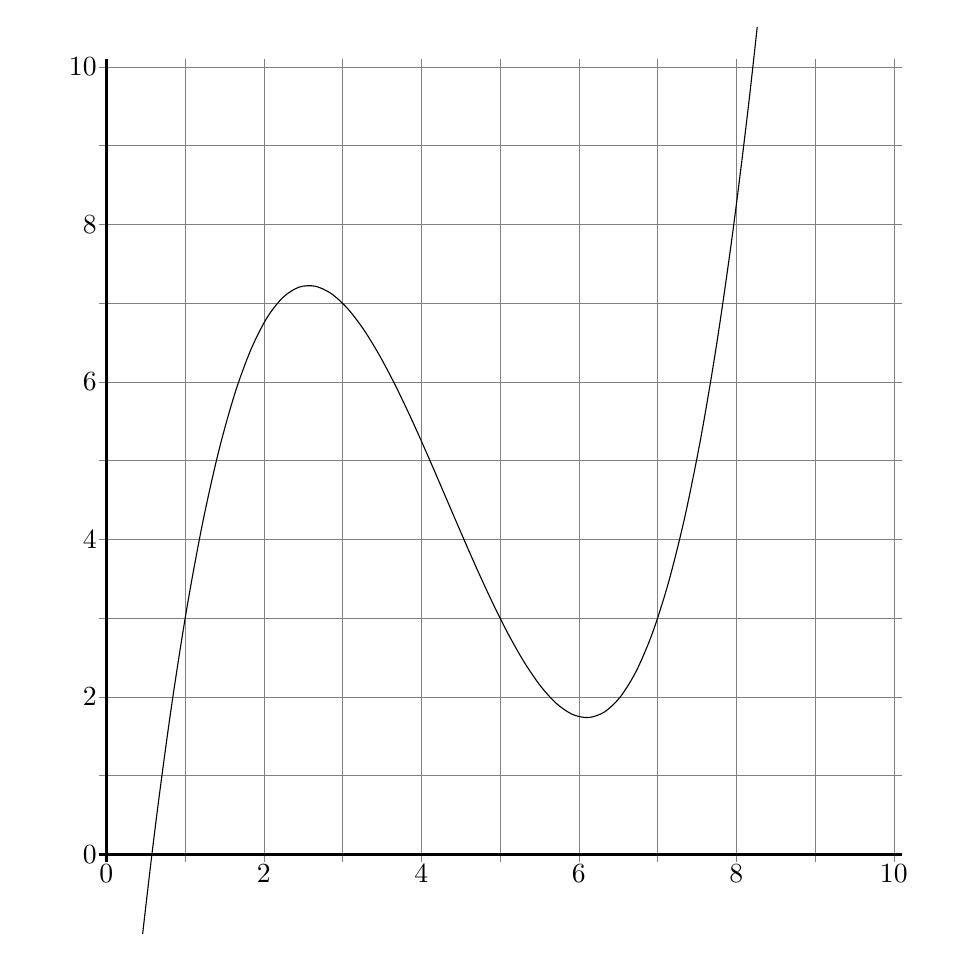
\begin{tikzpicture}
 \clip
 (-1,-1) rectangle (10.5,10.5)
 ;
 \draw[very thin,color=gray] (-0.1,-0.1) grid (10.1,10.1);
 \draw
 (0,0) node[below] {0}
 (2,0) node[below] {2}
 (4,0) node[below] {4}
 (6,0) node[below] {6}
 (8,0) node[below] {8}
 (10,0) node[below] {10}
 (0,0) node[left] {0}
 (0,2) node[left] {2}
 (0,4) node[left] {4}
 (0,6) node[left] {6}
 (0,8) node[left] {8}
 (0,10) node[left] {10}
 ;
 \draw[thick] (-0.1,0) -- (10.1,0);
 \draw[thick] (0,-0.1) -- (0,10.1);
 \draw
 plot[very thick, domain=0:10, range=0:10, smooth, samples=50]
 (\x, {0.25*(\x - 1)*(\x - 5)*(\x - 7) + 3})
 ;
\end{tikzpicture}

\begin{ProblemSet}[pencil space=0.75in]
 \begin{Problem}
  What is $f(3)$?
 \end{Problem}
 \begin{Problem}
  What are the solutions to $f(x) = 3$?
 \end{Problem}
 \begin{Problem}
  What is $f(4)$?
  Give an approximation to about the nearest tenth.
 \end{Problem}
 \begin{Problem}
  What are the solutions to $f(x) = 6$?
  Give an approximation to about the nearest tenth.
 \end{Problem}
\end{ProblemSet}

%%% Local Variables:
%%% mode: latex
%%% TeX-master: "Business-calculus-workbook"
%%% End:

\Section{Graph sketching---plotting points}

The graph of a function $f$ is a set of points in a coordinate plane.
We usually associate the horizontal axis with an independent variable, typically $x$, and the vertical axis with a dependent variable, typically $y$, and label the graph $y = f(x)$.
Each number $x$ in the domain of $f$ corresponds to a point $(x, f(x))$.

Consider the function
\begin{equation*}
 f(x) = -\frac{1}{5} x^2 (x - 4)
\end{equation*}
\begin{ProblemSet}[pencil space=0.5in]
 \begin{Problem}[pencil space=0in]
  Find the coordinates of the points on the graph of $f$ whose $x$-coordinates are $-2$, $-1$, $0$, $1$, $2$, $3$, $4$, $5$.
  List them in this table.
  Round the $y$-coordinates to the nearest tenth.

  \begin{tikzpicture}
   \path[use as bounding box] (-1,-1) rectangle (9,10);
   \draw[color=GraphingGridColor, line width=\GraphingGridLineWidth,
   ]
   (0, 0) grid[xstep=4,ystep=1] (8, 8)
   ;
   \node at (2,8.5) {$x$};
   \node at (6,8.5) {$f(x)$};
  \end{tikzpicture}
 \end{Problem}
 \begin{Problem}
  Choose an $x$-range, that is, a number $\xMin$ a bit less than all those $x$-values and a number $\xMax$ a bit greater than all those $x$-values.
 \end{Problem}
 \begin{Problem}
  Choose a $y$-range, that is, a number $\yMin$ a bit less than all those $y$-values and a number $\yMax$ a bit greater than all those $y$-values.
 \end{Problem}
 \begin{Problem}
  Draw axes on the grid below and set up a coordinate system that includes the interval from $\xMin$ to $\xMax$ horizontally, and $\yMin$ to $\yMax$ vertically.
  Draw tick marks and numbers on the axes to indicate the scale.
  The horizontal and vertical scales don't have to be the same and you don't have to use the whole grid.
  Then plot the points you wrote down in the table and draw a smooth curve connecting them.
  Use a calculator to check your picture.

  \bigskip
  \GraphingGrid
 \end{Problem}
 \begin{Problem}
  Use the graph to estimate $f(1.5)$ and check it with your calculator.
 \end{Problem}
 \begin{Problem}
  Use the graph to estimate the three solutions to $f(x) = 1$ and check them with your calculator.
 \end{Problem}
\end{ProblemSet}

%%% Local Variables:
%%% mode: latex
%%% TeX-master: "Business-calculus-workbook"
%%% End:

\Section{Algebra practice---solving}

Solve the following equations for the unknown variable.
You may need to do some simplifications as you solve.
Expect to use lots of inverse operations.
(This is sometimes called ``peeling the onion.'')
Your final answer should be an integer or a rational number.
Improper fractions, as in $\nicefrac{5}{2}$, are okay.

\begin{multicols}{2}
 \begin{ProblemSet}[pencil space=3.5in]
  \EqProb{6x + 2 = 4x - 1}
  \EqProb{\frac{2 + 2q}{3} = \frac{1}{2} q}

  \EqProb{\frac{1}{x} + \frac{1}{2} = 3}

  \EqProb{5 = \sqrt{16 - x}}
 \end{ProblemSet}
\end{multicols}

\newpage

Solve these and give decimal approximations to the nearest thousandth, as in $0.123$ or $1.234$.

\begin{ProblemSet}[pencil space=3.5in]
 \EqProb{3.20 x + 0.75 = 122.85}
 \EqProb{\frac{3.38}{2.2 t - 0.5} = 0.09}
\end{ProblemSet}


\newpage
\Subheading{Extra practice}

Solve these in the same way.

\begin{multicols}{2}
 \begin{ProblemSet}[pencil space=0in]
  \EqProb{-3 t + 4 = 7 - t}
  \EqProb{3r + \frac{1}{2} = \frac{2r}{5} - 2}

  \EqProb{\frac{2}{3 - t} = \frac{5}{4}}
  \EqProb{\frac{b}{1 + b} = 2}
  \EqProb{-\frac{2}{5} = 1 + \frac{4}{3u}}

  \EqProb{3 \sqrt{9 + w} = 7}
  \EqProb{3 \sqrt{v} - 5 = 1}
  \EqProb{\frac{3}{\sqrt{q}} - 5 = 1}
 \end{ProblemSet}
\end{multicols}

%%% Local Variables:
%%% mode: latex
%%% TeX-master: "Business-calculus-workbook"
%%% End:

\Section{Properties of exponents for real numbers}

In the notation $a^n$, the number $a$ is called the \emph{base}, and the number $n$ is called the \emph{exponent} or \emph{power}.
A whole number exponent $n$ means repeated multiplication:
\begin{equation*}
 a^n \text{ means } \overbrace{a \times a \times \cdots \times a}^{\text{multiply $n$ copies of $a$}}
\end{equation*}
The meaning of a fractional exponent $n$ is given in \cref{sec:roots-frac-exp}.

The following properties hold as long as all operations are defined.

\begin{multicols}{2}

 \begin{FormulaBox}{Easy cases}
  \begin{equation*}
   \begin{split}
     a^0 &= 1  \text{ provided $a \neq 0$ }
     \\
     a^1 &= a
     \\
     a^2 &= a \cdot a
     \\
   \end{split}
  \end{equation*}
 \end{FormulaBox}

 \begin{FormulaBox}{Powers of $1$}
  \begin{equation*}
   1^n = 1
  \end{equation*}
 \end{FormulaBox}

 \begin{FormulaBox}{Powers of $0$}
  \begin{equation*}
   0^n =
   \begin{cases}
     0 & \text{ if $n > 0$}
     \\
     \text{undefined} & \text{ if $n \leq 0$ }
   \end{cases}
  \end{equation*}
 \end{FormulaBox}

 \begin{FormulaBox}{Sign of odd powers}
  If $n$ is \emph{odd}, $a^n$ has the same sign as $a$.
 \end{FormulaBox}

 \begin{FormulaBox}{Sign of even powers}
  If $n$ is \emph{even}, $a^n \geq 0$ no matter what sign $a$ has.
  In this case, $a^n = \Abs{a^n} = \Abs{a}^n$.
 \end{FormulaBox}

 \begin{FormulaBox}{Nested powers}
  \begin{equation*}
   (a^n)^m = a^{n \cdot m}
  \end{equation*}
 \end{FormulaBox}

 \begin{FormulaBox}{Product with same base}
  \begin{equation*}
   a^m \cdot a^n = a^{m+n}
  \end{equation*}
 \end{FormulaBox}

 \begin{FormulaBox}{Product with same exponent}
  \begin{equation*}
   a^n \cdot b^n = (a \cdot b)^n
  \end{equation*}
 \end{FormulaBox}

 \begin{FormulaBox}{Negative exponent}
  As long as $a \neq 0$:
  \begin{equation*}
   \begin{split}
     a^{-1} &= \frac{1}{a}
     \\
     a^{-n} &= \frac{1}{a^n}
     \\
     \frac{c}{a^n} &= c \cdot a^{-n}
     \\
   \end{split}
  \end{equation*}
 \end{FormulaBox}

 \begin{FormulaBox}{Quotient with same base}
  \begin{equation*}
   \frac{a^m}{a^n} = a^m \cdot a^{-n} = a^{m-n}
  \end{equation*}
 \end{FormulaBox}

 \begin{FormulaBox}{Quotient with same exponent}
  As long as $b \neq 0$:
  \begin{equation*}
   \frac{a^n}{b^n} = \pfrac{a}{b}^n
  \end{equation*}
 \end{FormulaBox}

\end{multicols}

%%% Local Variables:
%%% mode: latex
%%% TeX-master: "Business-calculus-workbook"
%%% End:

\Subheading{Algebra practice---simplifying with exponents}

Rewrite each of the following equations into a properly-formed equation of the form $z = $ a power of $x$.
That is, your answer should look like
\begin{equation*}
 z = x^B \text{ where $B$ is an integer or fraction}
\end{equation*}
Assume that $x$ is positive.
You can also write $1$ for $x^0$.

\begin{multicols}{2}
 \begin{ProblemSet}[pencil space=1in]
  \EqProb{z = x \cdot x}
  \EqProb{z = x \cdot x \cdot x}
  \EqProb{z = x \cdot x \cdot x \cdot x}
  \EqProb{z = x^2 \cdot x^4}
  \EqProb{z = \left(x^2 \cdot x\right)^4}
  \EqProb{z = \frac{x^2}{x^4}}
  \EqProb{z = \frac{x^4}{x^2}}
  \EqProb{z = \frac{x}{1}}
  \EqProb{z = \frac{1}{x}}
  \EqProb{z = \frac{1}{x} \cdot \frac{1}{x}}
  \EqProb{z = \frac{1}{x} \cdot \frac{1}{x} \cdot \frac{1}{x}}
  \EqProb{z = \frac{1}{x \cdot x}}
  \EqProb{z = \frac{1}{x \cdot x \cdot x}}
  \EqProb{z = \frac{1}{x^2}}
  \EqProb{z = \frac{1}{x^{-1}}}
  \EqProb{z = \pfrac{1}{x}^{-1}}
  \EqProb{z = \pfrac{1}{x^{-1}}^{-1}}
  \EqProb{z = \frac{\quad x \quad}{\frac{1}{x}}}
  \EqProb{z = \frac{\quad\frac{1}{x}\quad}{x}}
  \EqProb{z = \frac{\quad\frac{1}{x}\quad}{\frac{1}{x}}}
  \EqProb{z = \frac{\quad\frac{1}{x^3}\quad}{\pfrac{1}{x}^4}}
  \EqProb{z = \frac{\quad\frac{1}{x^3}\quad}{\frac{1^4}{x}}}
 \end{ProblemSet}
\end{multicols}

\newpage

Rewrite each of the following equations into a properly-formed equation of the form $z = $ a product of a constant, a power of $x$, and a power of $y$.
That is, your answer should look like
\begin{equation*}
 z = A x^B y^C \text{ where $A$, $B$, and $C$ are integers or fractions}
\end{equation*}
The constant factor $A$ and exponents $B$ and $C$ may be positive or negative.
In your answer, you can leave out multiplication by $1$ or an exponent of $1$.
Assume that $x$ and $y$ are positive.

\begin{multicols}{2}
 \begin{ProblemSet}[pencil space=2in]
  \EqProb{z = 6 \cdot x^3 \cdot x^2 \cdot y^{-1} \cdot y^3}
  \EqProb{z = 2 \cdot (x^2 \cdot y^2)^3}
  \EqProb{z = \frac{\left(x^2 \cdot y^{-3}\right)^2}{y^5 \cdot x^3}}
  \EqProb{z = \pfrac{4 x}{y} \cdot \pfrac{2 y}{x^{-1}}^2}
  \EqProb{z = \bigg(x \cdot (-2 \cdot y \cdot x^{-2}) \cdot y\bigg)^{-2}}

  \begin{Problem}
   \Large
   \begin{LeftEquation}
    z = \frac{\quad\frac{3 x^2}{y}\quad}{\quad\frac{2y^2}{x^{-3}}\quad}
   \end{LeftEquation}
  \end{Problem}

 \end{ProblemSet}
\end{multicols}

\newpage
\Subheading{Extra practice}

Simplify these in the same way.

\begin{multicols}{2}
 \begin{ProblemSet}[pencil space=0in]
  \EqProb{z = (2 \cdot x^2 \cdot y^2)^3}
  \EqProb{z = \frac{x^5 \cdot y^2}{x^3 \cdot y^4}}
  \EqProb{z = x^3 \cdot x^5 \cdot y^{-3} \cdot 8 \cdot \left(x \cdot y\right)^2}
  \EqProb{z = \left(\left(x^2 y\right)^3\right)^{-1}}
  \EqProb{z = \frac{1}{\left(\left(x^2 y\right)^3\right)^{-1}}}
  \EqProb{z = \left(\frac{3}{2} x^{\nicefrac{1}{2}} y\right)^{-3} x^{-\nicefrac{5}{2}}}

  \EqProb{z = \frac{5 x y^2}{5 x^2 y}}
  \EqProb{z = \frac{5 x y^2}{(5 x)^2 y}}
  \EqProb{z = \frac{5 (x y)^2}{(5 x)^2 y}}
  \EqProb{z = \frac{(5 x y)^2}{(5 x)^2 y}}
  \EqProb{z = \frac{(5 x y)^2}{5 x^2 y}}
  \EqProb{z = \pfrac{5 x y}{5 x^2 y}^2}
  \EqProb{z = \frac{\frac{(5 x y)^2}{5 x^2 y}}{\pfrac{5 x y}{5 x^2 y}^2}}
 \end{ProblemSet}
\end{multicols}

%%% Local Variables:
%%% mode: latex
%%% TeX-master: "Business-calculus-workbook"
%%% End:

\Section{Roots and fractional exponents}
\label{sec:roots-frac-exp}

\Subheading{Meaning of the root symbol for real numbers}

The principal $n$-th root of a real number $a$, written
$\sqrt[n]{a}$,
is the real number $z$ that solves
$z^n = a$ and has the same sign as $a$.
The term \emph{radical} is a synonym for the root symbol.
The number $a$ is called the \emph{radicand}.
The number $n$ is called the \emph{index} or \emph{degree} of the root.
We generally require the index to be \emph{positive}.

A plain root symbol $\sqrt{a}$ means the square root $\sqrt[2]{a}$.

The 3rd root $\sqrt[3]{a}$ is also called the cube root.

Be careful where you put the index:
\begin{equation*}
 \sqrt[3]{a} \text{ means the cube root of $a$}
\end{equation*}
But
\begin{equation*}
 3 \sqrt{a} \text{ means } 3 \times \sqrt{a}
\end{equation*}

\Subheading{Odd roots}

If $n$ is \emph{odd}, every real number $a$ has exactly one real $n$-th root $\sqrt[n]{a}$.
It has the same sign as $a$.

\Subheading{Even roots}

If $n$ is \emph{even}, things are more complicated.
\begin{itemize}
\item The equation $z^n = 0$ has only one solution, $z = 0$.
 So $\sqrt[n]{0} = 0$.

\item If $a > 0$, the equation $z^n = a$ has two solutions for $z$.
 The positive solution is $\sqrt[n]{a}$.
 The negative solution is $-\sqrt[n]{a}$.
 The set of two solutions is abbreviated $\pm \sqrt[n]{a}$.

\item If $a < 0$, there is no real solution to $z^n = a$, so for our purposes, $\sqrt[n]{a}$ is undefined.
\end{itemize}

Assuming $\nicefrac{m}{n}$ is in lowest terms,
\begin{equation*}
   a^{\nicefrac{m}{n}}
   = \left(\sqrt[n]{a}\right)^m
   = \sqrt[n]{a^m}
\end{equation*}
This definition only works under certain conditions:
\begin{itemize}
\item If $\frac{m}{n} > 0$:
 \begin{itemize}
 \item If $n$ is odd, this works for all real numbers $a$.
 \item If $n$ is even, this works for $a \geq 0$.
 \end{itemize}
\item If $\frac{m}{n} < 0$:
 \begin{itemize}
 \item If $n$ is odd, this works for $a \neq 0$.
 \item If $n$ is even, this works for $a > 0$.
 \end{itemize}
\end{itemize}

\Subheading{Special cases of nested even root and even power}

If $m$ and $n$ are both even and positive:
\begin{itemize}
\item This works for all $a$, even if $a < 0$:
 \begin{equation*}
  \sqrt[n]{a^m} = \sqrt[n]{\Abs{a}^m} = \Abs{a}^{\nicefrac{m}{n}}
 \end{equation*}
 However, this can only work for $a \geq 0$:
 \begin{equation*}
  \left(\sqrt[n]{a}\right)^m = a^{\nicefrac{m}{n}}
 \end{equation*}
\item In particular, $\sqrt{a^2} = \Abs{a}$ for every real $a$.
\item But $(\sqrt{a})^2$ is only real if $a \geq 0$, in which case $(\sqrt{a})^2 = a$.
\end{itemize}

If the exponent $n$ irrational, the power $a^n$ is only defined for $a \geq 0$ and must be defined in terms of logarithms.

\Subheading{Properties of roots}

The following properties hold as long as all operations are defined.

\begin{multicols}{2}

 \begin{FormulaBox}{Convert roots $\longleftrightarrow$ powers}
  \begin{equation*}
   \begin{split}
     \sqrt[n]{a} &= a^{\nicefrac{1}{n}}
     \\
     \frac{1}{\sqrt[n]{a}} &= \frac{1}{a^{\nicefrac{1}{n}}} = a^{-\nicefrac{1}{n}}
     \\
   \end{split}
  \end{equation*}
 \end{FormulaBox}

 \begin{FormulaBox}{Product with same index}
  \begin{equation*}
   \left(\sqrt[n]{\vphantom{b}a}\right)
   \cdot
   \left(\sqrt[n]{b}\right) = \sqrt[n]{a \cdot b}
  \end{equation*}
 \end{FormulaBox}

 \begin{FormulaBox}{Quotient with same index}
  \begin{equation*}
   \frac{\sqrt[n]{a}}{\sqrt[n]{b}}
   =
   \sqrt[n]{\frac{a}{b}}
  \end{equation*}
 \end{FormulaBox}

 \begin{FormulaBox}{Nested roots}
  \begin{equation*}
   \sqrt[m]{\sqrt[n]{a}} = \sqrt[m\cdot n]{a}
  \end{equation*}
 \end{FormulaBox}


\end{multicols}

%%% Local Variables:
%%% mode: latex
%%% TeX-master: "Business-calculus-workbook"
%%% End:

\Section{Algebra practice---simplifying with exponents and roots}

Rewrite each of the following equations into a properly-formed equation of the form $z = $ a product of a constant, a power of $x$, and a power of $y$.
That is, your answer should look like
\begin{equation*}
 z = A x^B y^C \text{ where $A$, $B$, and $C$ are integers or fractions}
\end{equation*}
The constant factor $A$ and exponents $B$ and $C$ may be positive or negative.
In your answer, you can leave out multiplication by $1$ or an exponent of $1$.
Assume that $x$ and $y$ are positive.

\begin{multicols}{2}
 \begin{ProblemSet}[pencil space=2in]

  \EqProb{z = \sqrt{9 x y}}
  \EqProb{z = 9 \sqrt{x y}}
  \EqProb{z = \sqrt{\frac{9 x}{y}}}
  \EqProb{z = \sqrt{16 x^3 y^{-5}}}

  \begin{Problem}[pencil space=4in]
   \Large
   \begin{LeftEquation}
    z = \frac{3 \sqrt[5]{x y^{-1}}}{x^{-1} y^2}
   \end{LeftEquation}
  \end{Problem}

 \end{ProblemSet}
\end{multicols}


\newpage
\Subheading{Extra practice}

Simplify these in the same way.
\begin{multicols}{2}
 \begin{ProblemSet}[pencil space=0in]

  \EqProb{z = \sqrt{\frac{1}{9 x y}}}
  \EqProb{z = \frac{1}{\sqrt{9 x y}}}
  \EqProb{z = \frac{1}{9 \sqrt{x y}}}
  \EqProb{z = \frac{9}{\sqrt{x y}}}
  \EqProb{z = 9 \cdot \sqrt{\frac{x}{y}}}
  \EqProb{z = \sqrt{\frac{x y}{9}}}
  \EqProb{z = \frac{\sqrt{x y}}{9}}
  \EqProb{z = \frac{y}{x \sqrt{9}}}
  \EqProb{z = \frac{y}{\sqrt{9 x}}}
  \EqProb{z = \frac{y}{9 \sqrt{x}}}
  \EqProb{z = \left(\sqrt{4 x}\right)\left(9 \sqrt{y}\right)}

  \begin{Problem}
   \Large
   \begin{LeftEquation}
    z = \sqrt{9 x \sqrt{16 y}}
   \end{LeftEquation}
  \end{Problem}

  \begin{Problem}
   \Large
   \begin{LeftEquation}
    z = \frac{\sqrt{\frac{y}{x}}}{5 x y}
   \end{LeftEquation}
  \end{Problem}

  \begin{Problem}
   \Large
   \begin{LeftEquation}
    z = \frac{4 x^{\nicefrac{3}{2}} y}{\sqrt[3]{-8 x^4 y}}
   \end{LeftEquation}
  \end{Problem}

 \end{ProblemSet}
\end{multicols}

%%% Local Variables:
%%% mode: latex
%%% TeX-master: "Business-calculus-workbook"
%%% End:

\Section{Algebra practice---solving quadratic equations}

\begin{multicols}{2}

 Quadratic equations can have zero, one, or two real solutions.
 (We won't be using complex number solutions in this course.)
 You can solve quadratic equations by factoring or using the quadratic formula.
 Always put the equation in standard form before trying to solve it.
 Factoring is usually easier, but it requires some trial \& error and it doesn't always work.
 The quadratic formula always works (even if the equation factors), but there are many opportunities to make mistakes while using it.
 If there's no degree 1 term, you can solve by inverse operations (peeling the onion) but factoring and the quadratic formula work as well.

 Solve these equations using whatever method you like.
 If an equation has only complex solutions, just write ``no real solutions.''

 \columnbreak

 \begin{FormulaBox}{Quadratic formula}
  The solutions to a quadratic equation in standard form
  \begin{equation*}
   a x^2 + b x + c = 0
  \end{equation*}
  are
  \begin{equation*}
   \frac{
    -b \pm \sqrt{b^2 - 4 a c}
   }{
    2 a
   }
  \end{equation*}
  If the part under the root symbol $b^2 - 4ac$ comes out negative, there are no real solutions.
 \end{FormulaBox}
\end{multicols}

\begin{multicols}{2}
 \begin{ProblemSet}[pencil space=2.5in]
  \EqProb{x^2 + 4x + 3 = 0}
  \EqProb{x^2 - x + 6 = 0}
  \EqProb{-2 x^2 + 6 x + 3 = 0}
  \EqProb{3 x^2 - 4x = 0}
  \EqProb{x \cdot (x + 4) = 8 - x}
  \EqProb[pencil space=3.5in]{u^2 - 5 u + 6 = -2 u^2 + 2 u - 1}
 \end{ProblemSet}
\end{multicols}

Solve, giving decimal approximations to the nearest thousandth, as in 0.123 or 1.234.

\begin{ProblemSet}[pencil space=3in]
 \EqProb{0.2 x^2 - 3.7 x + 1.2 = 0}
\end{ProblemSet}

\newpage
\Subheading{Extra practice}

Solve these in the same way.

\begin{multicols}{2}
 \begin{ProblemSet}[pencil space=0in]
  \EqProb{x^2 + 2x + 1 = 0}
  \EqProb{x^2 - 2x - 1 = 0}
  \EqProb{x^2 - x + 3 = 0}
  \EqProb{x^2 - x - 3 = 0}
  \EqProb{x^2 + x + 6 = 0}
  \EqProb{x^2 + 5 x + 6 = 0}
  \EqProb{x^2 - 5x + 6 = 0}
  \EqProb{x^2 + x - 12 = 0}
  \EqProb{x^2 + x + 12 = 0}
  \EqProb{x^2 + 8x + 15 = 0}
  \EqProb{2 x^2 + 4 x + 2 = 0}
  \EqProb{2 x^2 + 6 x + 3 = 0}
  \EqProb{2 x^2 + 6 x - 3 = 0}
  \EqProb{2 x^2 - 6 x + 3 = 0}
  \EqProb{x^2 - 1 = 0}
  \EqProb{x^2 + 1 = 0}
  \EqProb{5 x^2 - 2 = 0}
  \EqProb{-2x^2 - 8x = 0}
  \EqProb{x^2 + 1 = 2x}
  \EqProb{-t^2 + 3t = 4}
  \EqProb{r^2 + 5r + 6 = 4}
  \EqProb{-7w + 6 = -2w^2 + 3}
  \EqProb{-0.01 x^2 + 5.25 x - 48.5 = 0}
  \EqProb{\frac{1}{x} + \frac{1}{x + 1} = 2}
 \end{ProblemSet}
\end{multicols}

%%% Local Variables:
%%% mode: latex
%%% TeX-master: "Business-calculus-workbook"
%%% End:

\Section{Business modeling---core concepts}

There is a standard way to use functions to model a business.
Be sure you understand the conceptual meaning of the symbols used in this setup.

\begin{ProblemSet}
 \begin{Problem}
  In common speech, the terms \emph{cost} and \emph{price} can be used for the same meaning.
  However, in business scenarios, the terms \emph{cost} and \emph{price} have very different meanings.

  In a business context, what does \emph{price} mean?
 \end{Problem}
 \begin{Problem}
  In a business context, what does \emph{cost} mean?
 \end{Problem}
 \begin{Problem}
  In the context of a business scenario, the symbol $x$ usually means what?
  (And you'll have to read carefully:
  Every so often, $x$ gets used for something else, sorry, nothing I can do about it.)

  ``The symbol $x$ means \dots
 \end{Problem}
 \begin{Problem}
  Conceptually, the \emph{demand function} takes as its input a number that means what?
 \end{Problem}
 \begin{Problem}
  Conceptually, the \emph{demand function} produces as its output a number that means what?
 \end{Problem}
 \begin{Problem}
  Conceptually, the \emph{revenue function} takes as its input a number that means what?
 \end{Problem}
 \begin{Problem}
  Conceptually, the \emph{revenue function} produces as its output a number that means what?
 \end{Problem}
 \begin{Problem}
  Conceptually, the \emph{cost function} takes as its input a number that means what?
 \end{Problem}
 \begin{Problem}
  Conceptually, the \emph{cost function} produces as its output a number that means what?
 \end{Problem}
 \begin{Problem}
  Conceptually, the \emph{profit function} takes as its input a number that means what?
 \end{Problem}
 \begin{Problem}
  Conceptually, the \emph{profit function} produces as its output a number that means what?
 \end{Problem}

 \begin{Problem}
  Conceptually, how do you begin building a revenue function?
 \end{Problem}
 \begin{Problem}
  Conceptually, how do you begin building a profit function?
 \end{Problem}
 \begin{Problem}
  What equations do break-even points satisfy?
 \end{Problem}
\end{ProblemSet}

\newpage

Consider the following business scenario.
A jewelry shop sells a particular kind of bracelet.
Each bracelet costs the store $\$15.75$.
The manager estimates that to sell $x$ bracelets per week, the price of a bracelet should be $30.00 - 0.25 x$ dollars.

Answer the following, using equations for final answers whenever possible.
When the result is a number, give a decimal approximation to the nearest cent or hundredth of a unit.
When the result is a function, write an equation giving the function as a simplified, explicit expression, in terms of $x$, that does not reference other functions.

\begin{ProblemSet}
 \begin{Problem}
  Conceptually, what does the symbol $x$ represent?
 \end{Problem}
 \begin{Problem}
  Which function (demand, revenue, cost, profit), is given by the expression $30.00 - 0.25 x$?
 \end{Problem}
 \begin{Problem}
  The number $\$15.75$ is directly relevant to which function (demand, revenue, cost, profit)?
 \end{Problem}
 \begin{Problem}
  Build a formula for the cost function, $C(x) = \dots$
 \end{Problem}
 \begin{Problem}
  Build a formula for the demand function, $D(x) = \dots$
 \end{Problem}
 \begin{Problem}
  Build a formula for the revenue function, $R(x) = \dots$
 \end{Problem}
 \begin{Problem}
  Build a formula for the profit function, $P(x) = \dots$
 \end{Problem}
 \begin{Problem}
  How much does it cost the store to acquire $20$ bracelets?
 \end{Problem}
 \begin{Problem}
  If the store plans to sell $20$ bracelets per week, at what price should they be sold?
 \end{Problem}
 \begin{Problem}
  If the store sells $20$ bracelets per week, what is the weekly revenue?
 \end{Problem}
 \begin{Problem}
  If the store sells $20$ bracelets per week, what is the weekly profit?
 \end{Problem}
 \begin{Problem}
  If the store plans to sell bracelets for $\$22.00$, how many should they plan to sell on average each week?
  (It's okay for this to be a fractional amount.)
 \end{Problem}
 \begin{Problem}
  What are the two break-even points for this business?
 \end{Problem}
\end{ProblemSet}

\newpage

Here's another business scenario.

A factory produces screwdrivers. Suppose it costs
\begin{equation*}
 10.00 + 1.75 x \text{ dollars}
\end{equation*}
to produce $x$ screwdrivers.
If the price of a screwdriver is $\$8$, the manufacturer can sell $300$ of them per month.
However, they can only sell $250$ of them per month if the price is $\$10$.

Fully simplify all answers.
Give answers as equations using proper notation when possible.
Give decimal approximations to the nearest cent or hundredth of a unit.

\begin{ProblemSet}
 \begin{Problem}[pencil space=0.5in]
  On the following grid, set up axes that are appropriate for sketching the graph of the demand function.
  Label each axis with the concept that it represents.
  Plot two points based on the given information, and draw the line through these points.
  This line is the graph of the demand function.
  \vspace{0.5in}

  \GraphingGridSmall

 \end{Problem}

 \begin{Problem}
  Assuming the demand function is linear, build a formula for it.
  Write it as an equation $D(x) = \dots$
 \end{Problem}

 \begin{Problem}
  What is the cost function?
 \end{Problem}

 \begin{Problem}
  What is the revenue function?
 \end{Problem}

 \begin{Problem}
  What is the profit function?
 \end{Problem}

 \begin{Problem}
  At what price should screwdrivers be sold to sell $220$ per month?
 \end{Problem}

 \begin{Problem}
  How many will be sold if the price is $\$11.00$?
 \end{Problem}

 \begin{Problem}
  How much does it cost to produce $250$ screwdrivers per month?
 \end{Problem}

 \begin{Problem}
  What is the profit if $250$ screwdrivers are sold?
 \end{Problem}

 \begin{Problem}
  What are the break-even points for this business?
 \end{Problem}

\end{ProblemSet}

%%% Local Variables:
%%% mode: latex
%%% TeX-master: "Business-calculus-workbook"
%%% End:

\Section{Limits}

Consider the function
% ( (x - 5)(x + 5) ) / ( (x - 5)(x - 7) )
% (x^2 - 25) / (x^2 - 12x + 35)
\begin{equation*}
 f(x) = \frac{x^2 - 25}{x^2 - 12x + 35}
\end{equation*}
Enter $f$ as a function in your calculator.

\begin{ProblemSet}
 \begin{Problem}
  What is the domain of $f$?
  Hint: It should be all real numbers except for two numbers that must be excluded because they would result in division by zero.
 \end{Problem}
 \begin{Problem}[pencil space=2in]
  Pick one of the gaps in the domain of $f$.
  Use a calculator to evaluate $f$ near that value of $x$.
  (For example, if there's a gap at $x = 2$, then $f(2)$ is undefined, so look at $f(1.9)$, $f(1.99)$, \dots and $f(2.1)$, $f(2.01)$, \dots)
  Write down a table of $x$ and $y$ values.
  Does it look like $f$ approaches a limit at that value of $x$?
  If so, write an equation using limit notation for what you found.
  Otherwise, write that the limit does not exist.
 \end{Problem}
 \begin{Problem}[pencil space=2in]
  Do the same for the other gap.
 \end{Problem}
 \begin{Problem}
  Choose an $x$-range, that is, minimum and maximum values of $x$ that include the gaps and some space to the left and right.
  Write it here.
 \end{Problem}
 \begin{Problem}
  Use a calculator to sketch the graph of $f$ using the $x$-range you just found.
  Select a $y$-range that lets you see all the interesting features of $f$.
  Sketch the graph on the grid below.
  Label the axes.
  Draw a dotted line $\vdots$ for the vertical asymptote.
  Draw a small circle $\circ$ for the missing point.
  \bigskip

  \GraphingGrid
 \end{Problem}
 \begin{Problem}[pencil space=3in]
  Now you'll use an algebraic method to confirm the numerical results.
  Factor the numerator and denominator of $f$.
  Cancel common factors.
  Write an equation defining $f^*(x) =$ this simplified expression.
 \end{Problem}
 \begin{Problem}
  What is the domain of $f^*$?
  Hint: It should have only one gap.
 \end{Problem}
 \begin{Problem}[pencil space=2in]
  The domain of $f^*$ includes one value of $x$ that is not in the domain of $f$, so the limit of $f$ exists at that number, even though $f$ is not defined at that number.
  Use $f^*$ to compute the value of the limit.
  Express what you found using limit notation.
 \end{Problem}
\end{ProblemSet}

%%% Local Variables:
%%% mode: latex
%%% TeX-master: "Business-calculus-workbook"
%%% End:

\Section{Derivative rules---basics}

\begin{multicols}{2}

 \begin{FormulaBox}{Derivative of just a constant}
  \Formula{\D{\K}}{0}
 \end{FormulaBox}

 \begin{FormulaBox}{Derivative of addition of a constant}
  \Formula{\D{\Y + \K}}{\D{\Y}}
 \end{FormulaBox}

 \begin{FormulaBox}{Derivative of multiplication by a constant}
  \Formula{\D{\K \cdot \Y}}{\K \cdot \D{\Y}}
 \end{FormulaBox}

 \columnbreak

 \begin{FormulaBox}{Derivative of addition in general}
  \Formula{\D{\U+\V}}{\D{\U} + \D{\V}}
 \end{FormulaBox}

 \begin{FormulaBox}{Derivative of subtraction in general}
  \Formula{\D{\U-\V}}{\D{\U} - \D{\V}}
 \end{FormulaBox}

 \begin{FormulaBox}{Derivative of variable to a constant power}
  \Formula{\D{\X^\P}}{\P \cdot \X^{\P - 1}}
 \end{FormulaBox}

\end{multicols}

%%% Local Variables:
%%% mode: latex
%%% TeX-master: "Business-calculus-workbook"
%%% End:

\Section{Derivative practice---basics}

\begin{ProblemSet}

 \begin{Problem}
  What is $f'(x)$?
  \begin{equation*}
   f(x) = 3 x + 7
  \end{equation*}
 \end{Problem}

 \begin{Problem}
  What is $g'(x)$?
  \begin{equation*}
   g(x) = x^3 + x^4
  \end{equation*}
 \end{Problem}

 \begin{Problem}
  What is $h'(x)$?
  \begin{equation*}
   h(x) = 10 x^3 - x^4
  \end{equation*}
 \end{Problem}

 \begin{Problem}
  What is $u'(t)$?
  \begin{equation*}
   u(t) = 5 \left(t^3 + t^4\right)
  \end{equation*}
 \end{Problem}

 \begin{Problem}
  What is $v'(t)$?
  \begin{equation*}
   v(t) = \left(t^5 - 8 t\right) \times 4
  \end{equation*}
 \end{Problem}

 \begin{Problem}
  What is $w'(t)$?
  \begin{equation*}
   w(t) = t^{-4}
  \end{equation*}
 \end{Problem}

 \begin{Problem}
  What is $p'(z)$?
  \begin{equation*}
   p(z) = \sqrt{z}
  \end{equation*}
 \end{Problem}

 \begin{Problem}
  What is $q'(z)$?
  \begin{equation*}
   q(z) = \frac{1}{z}
  \end{equation*}
 \end{Problem}

 \begin{Problem}
  What is $r'(z)$?
  \begin{equation*}
   r(z) = \frac{1}{\sqrt{z}}
  \end{equation*}
 \end{Problem}

 \begin{Problem}
  What is $f'(x)$?
  \begin{equation*}
   f(x) = \frac{4}{x} + 6 \sqrt{x}
  \end{equation*}
 \end{Problem}

 \begin{Problem}
  What is $g'(x)$?
  \begin{equation*}
   g(x) = x (x + 1)
  \end{equation*}
 \end{Problem}

 \begin{Problem}
  What is $h'(w)$?
  \begin{equation*}
   h(w) = \frac{5 w^2 - 6 w^3}{w}
  \end{equation*}
 \end{Problem}

 \begin{Problem}
  What is $q'(x)$?
  \begin{equation*}
   q(x) = 16 \sqrt{x}
  \end{equation*}
 \end{Problem}

 \begin{Problem}
  What is $r'(x)$?
  \begin{equation*}
   r(x) = \sqrt{16 x}
  \end{equation*}
 \end{Problem}

 \begin{Problem}
  What is $m'(s)$?
  \begin{equation*}
   m(s) = 7 \sqrt{s}
  \end{equation*}
 \end{Problem}

 \begin{Problem}
  What is $n'(s)$?
  \begin{equation*}
   n(s) = \sqrt{7 s}
  \end{equation*}
 \end{Problem}

 \begin{Problem}
  What is $\Deriv{y}{x}$?
  \begin{equation*}
   y = 6 x^2 - 4 x + 10
  \end{equation*}
 \end{Problem}

 \begin{Problem}
  What is $\Deriv{p}{r}$?
  \begin{equation*}
   p = 10 - \frac{5}{r^2}
  \end{equation*}
 \end{Problem}

 \begin{Problem}
  What is $\Deriv{y}{x}$?
  \begin{equation*}
   y = x
  \end{equation*}
 \end{Problem}

 \begin{Problem}
  What is $\Deriv{u}{t}$?
  \begin{equation*}
   u = 42
  \end{equation*}
 \end{Problem}

 \begin{Problem}
  What is $\Deriv{w}{z}$?
  \begin{equation*}
   w = \sqrt{5}
  \end{equation*}
 \end{Problem}

 \begin{Problem}
  What is $\Deriv{b}{q}$?
  \begin{equation*}
   b = q^2 + 6^2 q + 5^2
  \end{equation*}
 \end{Problem}

 \begin{Problem}
  What is $r'(t)$?
  \begin{equation*}
   r(t) = \frac{t^2 + 5 t + 3}{2}
  \end{equation*}
 \end{Problem}

  \begin{Problem}
  What is $r'(t)$?
  \begin{equation*}
   u(t) = \frac{t^2 + 5 t + 3}{t}
  \end{equation*}
 \end{Problem}

\end{ProblemSet}

%%% Local Variables:
%%% mode: latex
%%% TeX-master: "Business-calculus-workbook"
%%% End:

\Section{Applications---rate of change}

You are traveling north on I-95 from Savannah.
After an early lunch, you drive at a constant speed, so that at noon, you are at mile marker 15.
At 12:30, you reach mile marker 50.

\begin{ProblemSet}
 \begin{Problem}[pencil space=0in]
  Plot your location, that is, the mile marker on I-95, as a function of time on this grid.
  Represent time as the number of hours since noon.
  Let time go up to at least 1:30.
  Be sure to label the axes and indicate the time scale and location scale.

  \bigskip
  \GraphingGridSmall

 \end{Problem}
 \begin{Problem}
  Since your speed is constant, your location $y$ is a linear function of time $t$.
  Write an equation $y = m t + b$ for your location as a function of time.
 \end{Problem}
 \begin{Problem}[pencil space=0.5in]
  What is your speed during this trip?
  What feature of the equation $y = m t + b$ does this number correspond to?
 \end{Problem}
 \begin{Problem}[pencil space=0.5in]
  At what time will you arrive at mile marker 190?
 \end{Problem}
\end{ProblemSet}

\newpage
The water level in a tidal creek is approximately
\begin{equation*}
 w(t) = 3 + 1.2 t - 0.08 t^2 \text{ feet}
\end{equation*}
where $t$ is time in hours from now.

\begin{ProblemSet}[pencil space=2in]
 \begin{Problem}
  What is the derivative of the water level as a function of time?
 \end{Problem}
 \begin{Problem}
  What will the water level be $4$ hours from now?
  Give your answer to the nearest thousandth.
 \end{Problem}
 \begin{Problem}
  What will the water level be $4.5$ hours from now?
  Give your answer to the nearest thousandth.
 \end{Problem}
 \begin{Problem}
  What is the \emph{average rate of change} of the water level over the time interval from $4$ to $4.5$ hours from now?
  Give your answer to the nearest thousandth.
 \end{Problem}
 \begin{Problem}
  At what \emph{instantaneous rate} with respect to time will the water level be changing $4$ hours from now?
  Give your answer to the nearest thousandth.
 \end{Problem}
\end{ProblemSet}

%%% Local Variables:
%%% mode: latex
%%% TeX-master: "Business-calculus-workbook"
%%% End:

\Section{Geometry---tangent lines}

Let's work with the following function.
\begin{equation*}
 f(x) = - \frac{1}{2} x^2 + 3x + 5
\end{equation*}
\begin{ProblemSet}
 \begin{Problem}
  There is one point on the graph of $f$ at which $x = -2$.
  Write this point as an ordered pair.
 \end{Problem}
 \begin{Problem}
  What is the derivative of $f$?
 \end{Problem}
 \begin{Problem}
  What is the instantaneous rate of change of $f$ with respect to $x$ at $x = -2$?
 \end{Problem}
 \begin{Problem}
  What is the slope of the line tangent to the graph of $f$ at $x = -2$?
 \end{Problem}
 \begin{Problem}
  Write an equation of the line tangent to the graph of $f$ at $x = -2$.
 \end{Problem}
 \begin{Problem}
  On the grid below, sketch the graph of $f$.
  Use your calculator to help.
  Use $\xMin = -10$, $\xMax = 10$, $\yMin = -30$, $\yMax = 30$.
  Then draw the line tangent to the graph of $f$ at $x = -2$.

  \bigskip
  \GraphingGridMedium
 \end{Problem}
\end{ProblemSet}

%%% Local Variables:
%%% mode: latex
%%% TeX-master: "Business-calculus-workbook"
%%% End:

\Section{Business modeling---marginal analysis}
\label{sec:biz-mod-marginal}

Recall that in a business scenario, \emph{marginal [thing]} is the derivative of [thing] with respect to the number of units of the product that are produced and sold.
Marginals approximate the change that would result if the business made an incremental change, that is, supposing it produced and sold one more unit of its product.

% For example, marginal cost is the derivative of the cost function with respect to the number of units produced.
% The notation for the marginal cost function is $C'(x)$.
% The exact change in the business's costs if it made that incremental change is $C(x+1) - C(x)$, and $C'(x) \approx C(x+1) - C(x)$.
% Marginal cost is approximately how much it would cost to produce and sell one additional unit after producing and selling $x$ units.

% It has to be a function of $x$:
% If our business has been selling only few units (small $x$), producing and selling one more might be inexpensive (small $C'(x)$).
% However, if our business has been selling many units (large $x$), producing and selling an additional unit might result in surprising new expenses, such the need to buy additional components from more expensive sources, paying workers overtime, and paying for more storage space (large $C'(x)$).

% Marginal revenue is $R'(x)$, and marginal profit is $P'(x)$.

Consider the following business scenario.
A jewelry shop sells a particular kind of necklace.
Each week, the shop can order $x$ of these necklaces from a wholesaler for $12.25 + 8.75 x$ dollars.
The manager estimates that to sell $x$ necklaces per week, the price of a necklace should be $25.00 - 0.25 x$ dollars.

Answer the following, using equations for final answers whenever possible.
When the result is a number, give a decimal approximation to the nearest cent or hundredth of a unit.
When the result is a function, write an equation giving the function as a simplified, explicit expression, in terms of $x$, that does not reference other functions.

\begin{ProblemSet}

 \begin{Problem}
  What is the demand function?
 \end{Problem}

 \begin{Problem}
  What is the cost function?
 \end{Problem}

 \begin{Problem}
  What is the revenue function?
 \end{Problem}

 \begin{Problem}
  What is the profit function?
 \end{Problem}

 \begin{Problem}
  What is the marginal cost function?
 \end{Problem}

 \begin{Problem}
  What is the marginal revenue function?
 \end{Problem}

 \begin{Problem}
  What is the marginal profit function?
 \end{Problem}

 \begin{Problem}[pencil space=4in]
  At what values of $x$ are the break-even points for this business?
 \end{Problem}

 \begin{Problem}
  What profit does the shop earn if they sell exactly enough necklaces to break even?
 \end{Problem}

 \begin{Problem}
  Suppose the shop sells exactly enough necklaces to break even.
  At what price will necklaces be sold to accomplish this?
  Give your answer to the nearest cent.
  (There are two prices because there are two break-even points.)
 \end{Problem}

\end{ProblemSet}

%%% Local Variables:
%%% mode: latex
%%% TeX-master: "Business-calculus-workbook"
%%% End:

\Section{Business modeling---average cost}
\label{sec:biz-mod-avg-cost}

\begin{ProblemSet}[pencil space=1in]
 \begin{Problem}
  Conceptually, the \emph{average cost function} takes as its input a number that means what?
 \end{Problem}
 \begin{Problem}
  Conceptually, the \emph{average cost function} produces as its output a number that means what?
 \end{Problem}
 \begin{Problem}
  If $C(x)$ is the cost function for a business, what is the general equation for the average cost function?
 \end{Problem}
 \begin{Problem}
  Suppose it costs $10 + 3x + 0.1 x^2$ dollars to produce a unit of a product.
  Sketch the average cost function, using an $x$-range of $0$ to $50$ and a $y$-range of $0$ to $20$.
  \bigskip

  \GraphingGridSmall
 \end{Problem}
\end{ProblemSet}

\newpage
Consider the following scenario.
Cougar Caf\'e sells muffins.
Based on past sales figures, the manager estimates that to sell $x$ packs of muffins per day, the price of a pack of muffins should be
\begin{equation*}
 20.0 - 0.12 x \text{ dollars }
\end{equation*}
The cost to make $x$ packs of muffins is
\begin{equation*}
 3 + 4.25 x + 0.09 x^2 \text{ dollars }
\end{equation*}


\begin{ProblemSet}[pencil space=1in]
 \begin{Problem}
  What is the cost function?
 \end{Problem}
 \begin{Problem}
  What is the marginal cost function?
 \end{Problem}
 \begin{Problem}[pencil space=2in]
  What is the average cost function?
 \end{Problem}
 \begin{Problem}[pencil space=2in]
  What is the marginal average cost function?
 \end{Problem}
\end{ProblemSet}

%%% Local Variables:
%%% mode: latex
%%% TeX-master: "Business-calculus-workbook"
%%% End:

\Section{Derivative rules---product and quotient}

\begin{FormulaBox}{Derivative of multiplication by a constant}
 \Formula{\D{\K \cdot \Y}}{\K \cdot \D{\Y}}
\end{FormulaBox}

\begin{FormulaBox}{Product rule---derivative of multiplication in general}
 \Formula{\D{\U \cdot \V}}{\D{\U} \cdot \V + \U \cdot \D{\V}}
\end{FormulaBox}

\begin{FormulaBox}{Quotient rule---derivative of division in general}
 \Formula{\D{\frac{\Hi}{\Lo}}}%
 {\frac{\D{\Hi}\cdot\Lo - \Hi\cdot\D{\Lo}}{\Lo^2}}
\end{FormulaBox}

%%% Local Variables:
%%% mode: latex
%%% TeX-master: "Business-calculus-workbook"
%%% End:

\Section{Derivative practice---product rule}

\begin{ProblemSet}[pencil space=2in]

 \begin{Problem}[pencil space=1in]
  What is $u'(x)$?
  \begin{equation*}
   \LeftStyle{u(x) = 6 x^2 - 4x + 7}
  \end{equation*}
 \end{Problem}

 \begin{Problem}[pencil space=1in]
  What is $v'(x)$?
  \begin{equation*}
   \RightStyle{v(x) = 3 x^2 + 2 x - 5}
  \end{equation*}
 \end{Problem}

 \begin{Problem}[pencil space=3in]
  What is $f'(x)$?
  \begin{equation*}
   f(x) =
   \LeftStyle{\left(6 x^2 - 4x + 7\right)}
   \RightStyle{\left(3 x^2 + 2 x - 5\right)}
  \end{equation*}
 \end{Problem}

 \begin{Problem}
  What is $g'(t)$?
  \begin{equation*}
   g(t) = \left(8 t^3 - 5t^2 + 3\right)\left(10t - t^2 + 4t^3\right)
  \end{equation*}
 \end{Problem}

 \begin{Problem}
  What is $h'(z)$?
  \begin{equation*}
   h(z) = (z^2+z)\cdot\left(-z^3 - 4z^2 + z\right)
  \end{equation*}
 \end{Problem}

 \begin{Problem}
  What is $k'(w)$?
  \begin{equation*}
   k(w) = \left(5w^2 - w^{-2}\right)\left(1 + \sqrt{2}\right)
  \end{equation*}
 \end{Problem}

 \begin{Problem}
  What is $g'(p)$?
  \begin{equation*}
   g(p) = \left(3\sqrt{p} + \frac{1}{\sqrt{7p}}\right)(5 p^2 + 9 p - 2)
  \end{equation*}
 \end{Problem}

\end{ProblemSet}

%%% Local Variables:
%%% mode: latex
%%% TeX-master: "Business-calculus-workbook"
%%% End:

\Section{Derivative practice---quotient rule}

\begin{ProblemSet}[pencil space=2in]

 \begin{Problem}[pencil space=1in]
  What is $u'(x)$?
  \begin{equation*}
   \LeftStyle{u(x) = 4 x^2 + 5 x - 10}
  \end{equation*}
 \end{Problem}

 \begin{Problem}[pencil space=1in]
  What is $v'(x)$?
  \begin{equation*}
   \RightStyle{v(x) = - x^2 - 7 x + 8}
  \end{equation*}
 \end{Problem}

 \begin{Problem}[pencil space=3in]
  What is $f'(x)$?
  \begin{equation*}
   f(x) = \frac{
    \LeftStyle{4 x^2 + 5 x - 10}
   }{
    \RightStyle{- x^2 - 7 x + 8}
   }
  \end{equation*}
 \end{Problem}

 \begin{Problem}
  What is $g'(t)$?
  \begin{equation*}
   g(t) = \frac{t^2 - 4t + 6}{t}
  \end{equation*}
 \end{Problem}

 \begin{Problem}
  What is $h'(w)$?
  \begin{equation*}
   h(w) = \frac{14}{3w^2 - w}
  \end{equation*}
 \end{Problem}

 \begin{Problem}
  What is $m'(q)$?
  \begin{equation*}
   m(q) = \frac{3q^2 - q}{14}
  \end{equation*}
 \end{Problem}

 \begin{Problem}
  What is $r'(z)$?
  \begin{equation*}
   r(z) = \frac{3z^{\nicefrac{7}{5}} + 4z}{5 - z + z^3}
  \end{equation*}
 \end{Problem}

\end{ProblemSet}

%%% Local Variables:
%%% mode: latex
%%% TeX-master: "Business-calculus-workbook"
%%% End:

\Section{Derivative rules---chain rule}

\begin{FormulaBox}{Chain rule, Lagrange notation}
 Given
 \begin{equation*}
  \begin{split}
    \OuterStyle{v(u)} &= \text{ \OuterStyle{function of $u$, \emph{outer function}} }
    \\
    \InnerStyle{u(x)} &= \text{ \InnerStyle{function of $x$, \emph{inner function}} }
    \\
    f(x) &= \OuterStyle{v\bigg(\InnerStyle{u(x)}\bigg)}
    \\
  \end{split}
 \end{equation*}
 Think of $f(x)$ as the composition of $\OuterStyle{v(u)}$ and $\InnerStyle{u(x)}$
 \begin{equation*}
  f'(x) = \OuterStyle{v'\bigg(\InnerStyle{u(x)}\bigg)}
  \cdot
  \InnerStyle{u'(x)}
 \end{equation*}
\end{FormulaBox}

\begin{FormulaBox}{Chain rule, Leibniz notation}
 Given
 \begin{equation*}
  \begin{split}
    y &= \text{ \OuterStyle{function of $u$, \emph{outer function}} }
    \\
    u &= \text{ \InnerStyle{function of $x$, \emph{inner function}} }
    \\
  \end{split}
 \end{equation*}
 Think of $y$ as a function of $x$
 \begin{equation*}
  \Deriv{y}{x} =
  \OuterStyle{\Deriv{y}{u}}
  \cdot
  \InnerStyle{\Deriv{u}{x}}
 \end{equation*}
\end{FormulaBox}

\begin{FormulaBox}{Chain rule, in words}
 \begin{equation*}
  \DerivWord{\Word{composition}}
  =
  \OuterStyle{\DerivWord{\Word{outer}}}\cdot\InnerStyle{\DerivWord{\Word{inner}}}
 \end{equation*}
\end{FormulaBox}

\begin{FormulaBox}{General power rule---combo power and chain}
 \Formula{\D{(\Y)^{\,\P}}}{\P \cdot (\Y)^{\,\P - 1} \cdot \D{\Y}}
\end{FormulaBox}

%%% Local Variables:
%%% mode: latex
%%% TeX-master: "Business-calculus-workbook"
%%% End:

\Section{Derivative practice---chain rule, Lagrange notation}

\begin{ProblemSet}[pencil space=2in]

 \begin{Problem}[pencil space=1in]
  What is $\OuterStyle{v'(u)}$?
  \begin{equation*}
   \OuterStyle{v(u) = \sqrt{u}}
  \end{equation*}
 \end{Problem}

 \begin{Problem}[pencil space=1in]
  What is $\InnerStyle{u'(x)}$?
  \begin{equation*}
   \InnerStyle{u(x) = 6 x^2 - 4x + 7}
  \end{equation*}
 \end{Problem}

 \begin{Problem}[pencil space=3in]
  What is $f'(x)$?
  \begin{equation*}
   f(x) = \OuterStyle{\sqrt{\InnerStyle{6 x^2 - 4x + 7}}}
  \end{equation*}
 \end{Problem}

  \begin{Problem}
  What is $g'(x)$?
  \begin{equation*}
   g(x) = \OuterStyle{\big(\InnerStyle{3 - 2x + 5x^2}\big)^2}
  \end{equation*}
 \end{Problem}

 \begin{Problem}
  What is $f'(x)$?
  \begin{equation*}
   f(x) = 4 \left(x^2 + 7\right)^5
  \end{equation*}
 \end{Problem}

 \begin{Problem}
  What is $f'(x)$?
  \begin{equation*}
   f(x) = \left(4 x^2 + 7\right)^5
  \end{equation*}
 \end{Problem}

 \begin{Problem}
  What is $f'(t)$?
  \begin{equation*}
   f(t) = \frac{1}{\sqrt{13 t}}
  \end{equation*}
 \end{Problem}

 \begin{Problem}
  What is $q'(t)$?
  \begin{equation*}
   q(t) = \left(t + \frac{3}{t}\right)^{\nicefrac{4}{3}}
  \end{equation*}
 \end{Problem}

 \begin{Problem}
  What is $h'(z)$?
  \begin{equation*}
   h(z) = 16 \left(z^4 - z^5\right)^{-5} - 7 z^{-3}
  \end{equation*}
 \end{Problem}

 % \begin{Problem}
 %  What is $p'(x)$?
 %  \begin{equation*}
 %   p(x) = 10 (3 x + 4)^{\nicefrac{2}{3}} + 8 \sqrt{5 - x^2} + \sqrt{7}
 %  \end{equation*}
 % \end{Problem}

\end{ProblemSet}

%%% Local Variables:
%%% mode: latex
%%% TeX-master: "Business-calculus-workbook"
%%% End:

\Section{Derivative practice---chain rule, Leibniz notation}


\begin{multicols}{2}
 Given
 \begin{equation*}
  \begin{split}
    \OuterStyle{y} &= \OuterStyle{2 u^2 + 4 u}
    \\
    \InnerStyle{u} &= \InnerStyle{-2 x^2 + 6x - 5}
  \end{split}
 \end{equation*}
 answer the following.
 \bigskip

 \begin{ProblemSet}[pencil space=1.25in]

  \begin{Problem}
   What is $\displaystyle{\Where{\OuterStyle{y}}{\InnerStyle{u=3}}}$?
  \end{Problem}

  \begin{Problem}
   What is $\displaystyle{\Where{\InnerStyle{u}}{x=2}}$?
  \end{Problem}

  \begin{Problem}
   What is $\displaystyle\Where{y}{x=2}?$
  \end{Problem}

  \begin{Problem}
   What is $\displaystyle{\InnerStyle{\Deriv{u}{x}}}$?
  \end{Problem}

  \begin{Problem}
   What is $\displaystyle{\Where{\InnerStyle{\Deriv{u}{x}}}{x=2}}$?
  \end{Problem}

  \begin{Problem}
   What is $\displaystyle{\OuterStyle{\Deriv{y}{u}}}$?
  \end{Problem}

  \begin{Problem}
   What is $\displaystyle{\Where{\OuterStyle{\Deriv{y}{u}}}{\InnerStyle{u=3}}}$?
  \end{Problem}

  \begin{Problem}
   What is $\displaystyle\Deriv{y}{x}$?
  \end{Problem}

  \begin{Problem}
   What is $\displaystyle\Where{\Deriv{y}{x}}{x=2}$?
  \end{Problem}

 \end{ProblemSet}
\end{multicols}

Given
\begin{equation*}
 \begin{split}
   y &= -u^3 + 2 u^2
   \\
   u &= x^2 - 3x - 2
 \end{split}
\end{equation*}
answer the following.
\bigskip

\begin{ProblemSet}[pencil space=2in]

 \begin{Problem}[pencil space=1in]
  What is $\displaystyle{\Where{y}{x=-2}}$?
 \end{Problem}

 \begin{Problem}
  What is $\displaystyle{\Deriv{y}{x}}$?
 \end{Problem}

 \begin{Problem}
  What is $\displaystyle{\Where{\Deriv{y}{x}}{x=-2}}$?
 \end{Problem}

\end{ProblemSet}

%%% Local Variables:
%%% mode: latex
%%% TeX-master: "Business-calculus-workbook"
%%% End:

\Section{Business modeling---harder functions}

Consider the following scenario.
Cougar Caf\'e sells cookies.
Based on past sales figures, the manager estimates that to sell $x$ packs of cookies, the price of a pack of cookies should be
\begin{equation*}
 55 \cdot \sqrt{1 - 0.02 x} \text{ dollars }
\end{equation*}
The cost to make $x$ packs of cookies is
\begin{equation*}
 4 + 3.50 x + 0.04 x^2 \text{ dollars }
\end{equation*}

\begin{ProblemSet}
 \begin{Problem}
  What is the revenue function?
 \end{Problem}
 \begin{Problem}[pencil space=2in]
  What is the marginal revenue function?
 \end{Problem}
 \begin{Problem}
  What is the cost function?
 \end{Problem}
 \begin{Problem}
  What is the marginal cost function?
 \end{Problem}
 \begin{Problem}
  What is the average cost function?
 \end{Problem}
 \begin{Problem}
  What is the marginal average cost function?
 \end{Problem}
 \begin{Problem}
  What is the profit function?
 \end{Problem}
 \begin{Problem}
  What is the marginal profit function?
 \end{Problem}
\end{ProblemSet}

%%% Local Variables:
%%% mode: latex
%%% TeX-master: "Business-calculus-workbook"
%%% End:

\Section{Visual intuition for graphs}

In each pair of grids, the upper grid shows the graph of $y = f(x)$.
Sketch the graph of $y = f'(x)$ on the grid below it.
Hint: Think about critical numbers.

{
\newcommand{\PicWidth}{3.25in}
\begin{tabular}{p{\PicWidth}p{\PicWidth}}
  \includegraphics[width=\PicWidth]{g1}
  & \includegraphics[width=\PicWidth]{g2}
  \\[0.25in]
  \includegraphics[width=\PicWidth]{g3}
  & \includegraphics[width=\PicWidth]{g4}
\end{tabular}
}

\newpage

In each pair of grids, the lower grid shows the graph of $y = f'(x)$.
Sketch a possible graph of $y = f(x)$ on the grid above it, assuming $f(0) = 0$.
Hint: Think about critical numbers.

{
\newcommand{\PicWidth}{3.25in}
\begin{tabular}{p{\PicWidth}p{\PicWidth}}
  \includegraphics[width=\PicWidth]{h1}
  & \includegraphics[width=\PicWidth]{h2}
  \\[0.25in]
  \includegraphics[width=\PicWidth]{h3}
  & \includegraphics[width=\PicWidth]{h4}
\end{tabular}
}

%%% Local Variables:
%%% mode: latex
%%% TeX-master: "Business-calculus-workbook"
%%% End:

\Section{Sketching graphs with the first derivative}
\label{sec:gr-with-fp}

Consider the function $f(x) = 2x^3 + 3x^2 - 120x + 200$.

\begin{ProblemSet}

 \begin{Problem}
  Find $f'(x)$
 \end{Problem}

 \begin{Problem}[pencil space=3in]
  Find critical numbers by solving $f'(x) = 0$.
  There should be two of them.
  Figure out which one is less than the other.
  Name the lesser one $c_1$ and the greater one $c_2$.
 \end{Problem}

 \begin{Problem}
  List out the open intervals between critical numbers.
  The first one goes from $-\infty$ to the least critical number.
  The second goes between the critical numbers.
  The third goes from the greatest critical number to $\infty$.
 \end{Problem}

 \newpage

 \begin{Problem}[pencil space=0in]
  Put marks on this number line for $c_1$ and $c_2$.
  Then mark three test numbers, one to the left of $c_1$,
  one between $c_1$ and $c_2$,
  and one to the right of $c_2$.
  There should be one test number from each interval you listed.

  \begin{tikzpicture}[scale=0.75]
   \clip (-11,-3) rectangle (11,3) ;
   \draw (-10.5,0) -- (10.5,0) ; %edit here for the axis
   \foreach \x in  {-10, -9, ..., 10} % edit here for the vertical lines
     \draw[shift={(\x,0)},color=black] (0pt,3pt) -- (0pt,-3pt);
   \foreach \x in {-10, -8, ..., 10} % edit here for the numbers
     \draw[shift={(\x,0)},color=black] (0pt,0pt) -- (0pt,-3pt) node[below] {$\x$};
  \end{tikzpicture}
 \end{Problem}

 \begin{Problem}[pencil space=0in]
  \begin{itemize}
  \item Enter the numbers you marked on the number line in the $x$ column, from least at the top to greatest at the bottom.
  \item Plug each of those values of $x$ into $f'$ and record that value in the $f'(x)$ column.
   There should be two boxes in the $f'$ column that are zero.
   The others should all be non-zero.
  \item For each test number, in the ``meaning'' column, write what the sign of $f'$ tells you about $f$ on the interval the test number came from.
  \item On the number line from before, draw increasing arrows $\nearrow$ and decreasing arrows $\searrow$ over the intervals where $f$ is increasing and decreasing.
  \item For each critical number, look at what happens in the interval just to its left and right, and determine what kind of critical point is there (local minimum, local maximum, neither).
   Write this in the ``meaning'' column on that row.
  \item On the number line from before, draw hills $\wedge$ and valleys $\vee$ over the critical numbers where $f$ has local maximum and local minimum points.
  \end{itemize}
  \bigskip

  \newcommand{\Bx}[1]{\Strut[-0.25in]{0.75in}#1}
  \begin{tabular}{l|p{1in}|p{1in}|p{3in}}
    Type & $x$ & $f'(x)$ & meaning
    \\ \hline
    \Bx{test} & & &
    \\ \hline
    \Bx{crit} & \Bx{$c_1 = $} & &
    \\ \hline
    \Bx{test} & & &
    \\ \hline
    \Bx{crit} & \Bx{$c_2 = $} & &
    \\ \hline
    \Bx{test} & & &
    \\ \hline
  \end{tabular}

 \end{Problem}

 \begin{Problem}[pencil space=2.5in]
  Write sentences to answer these questions:
  \begin{itemize}
  \item On what intervals is $f$ increasing?
  \item On what intervals is $f$ decreasing?
  \item At what coordinates $(x,y)$ does $f$ have local maximum points?
  \item At what coordinates $(x,y)$ does $f$ have local minimum points?
  \end{itemize}
 \end{Problem}

 \begin{Problem}
  On the grid below, sketch the graph of $f$ using the information that you've found.
  Draw axes and label the scales.
  Choose $\xMin$ a little to the left of $c_1$, and choose $\xMax$ a little to the right of $c_2$.
  Choose $\yMin$ a little below the $y$-value of the local minimum, and choose $\yMax$ a little above the $y$-value of the local maximum.
  That way, all important features of $f$ are visible.
  Plot the critical points you found and draw a smooth curve connecting them.
  The curve may be easier to draw if you plot a few extra points on the graph.
  Use the arrows on the number line as a guide.
  If you have conflicting information, look for a mistake and fix it.

  \bigskip
  \GraphingGrid

 \end{Problem}
\end{ProblemSet}

\newpage

Given the following function,
\begin{equation*}
 f(x) = -\frac{1}{3} x^3 - 2 x^2 + 12 x + 20
\end{equation*}
answer the following questions.
Give exact answers or decimal approximations to the nearest hundredth, as in $1.23$ or $12.34$.
For maximum credit, make appropriate use of differential calculus and show all your work.

\begin{itemize}
\item On what intervals is $f$ increasing, and on what intervals is $f$ decreasing?
\item Identify all critical points of $f$ (both coordinates), and classify each as a local maximum, a local minimum, or neither.
\item Draw the graph of $f$ on the given grid using this information.
 Be sure to label the axes.

\end{itemize}

\bigskip
\GraphingGrid

%%% Local Variables:
%%% mode: latex
%%% TeX-master: "Business-calculus-workbook"
%%% End:

\Section{Derivative practice---combinations and tricky ones}

\begin{ProblemSet}[pencil space=3in]

 \begin{Problem}
  What is $f'(x)$?
  \begin{equation*}
   f(x) = x^2 \left(x^2 + 3x\right)^{-2}
  \end{equation*}
 \end{Problem}

 \begin{Problem}
  What is $\Deriv{y}{t}$?
  \begin{equation*}
   y = \left(\frac{4t + 3}{t^2 - 1}\right)^{\nicefrac{3}{5}}
  \end{equation*}
 \end{Problem}

 \begin{Problem}
  What is $h'(z)$?
  \begin{equation*}
   h(z) = \frac{\left(z^5 - 4z\right)^{\nicefrac{1}{5}}}{5z - 3}
  \end{equation*}
 \end{Problem}

 \begin{Problem}
  What is $g'(t)$?
  \begin{equation*}
   g(t) = t\cdot(t+1)\cdot\left(3t^2 + 2\right)
  \end{equation*}
 \end{Problem}

\end{ProblemSet}

%%% Local Variables:
%%% mode: latex
%%% TeX-master: "Business-calculus-workbook"
%%% End:

\Section{Derivative practice---abstract functions}

In each of these problems, one function is defined in terms of another function.
The other function is not defined, so the final answer will include references to this other function or its derivative.
For clarity, Lagrange notation, as in $f(x)$, is used throughout.
A letter followed by an expression in parentheses, as in $f(x)$ or $w(t)$ will always mean function application, not multiplication.
Multiplication is always indicated by a dot $\cdot$ on this problem set.

\begin{ProblemSet}[pencil space=2.5in]

 \begin{Problem}
  What is $f'(x)$?
  Here, $g$ is a function.
  Your final answer will have $g$ and $g'$ in it.
  \begin{equation*}
   f(x) = x^2 \cdot g(x)
  \end{equation*}
 \end{Problem}

 \begin{Problem}[pencil space=3in]
  What is $g'(t)$?
  Here, $w$ is a function.
  Your final answer will have $w$ and $w'$ in it.
  \begin{equation*}
   g(t) = \frac{w(t) + t^2}{w(t) - t^2}
  \end{equation*}
 \end{Problem}

 \begin{Problem}
  What is $f'(x)$?
  Here, $m$ is a function.
  Your answer will $m'$ in it.
  \begin{equation*}
   f(x) = m\!\left(3\cdot x^2 + 7\right)
  \end{equation*}
 \end{Problem}

 \begin{Problem}
  What is $f'(x)$?
  Here, $q$ is a function.
  Your answer will have $q$ and $q'$ in it.
  \begin{equation*}
   f(x) = (10 + q(3\cdot x))^5
  \end{equation*}
 \end{Problem}

\end{ProblemSet}

%%% Local Variables:
%%% mode: latex
%%% TeX-master: "Business-calculus-workbook"
%%% End:

\Section{Absolute maximum and minimum}

Consider the function
\begin{equation*}
 f(x) = x^2 - 4x + 6
\end{equation*}
Suppose the domain of $f$ is restricted to the closed interval $[1,4]$.

\begin{ProblemSet}[pencil space=1in]
 \begin{Problem}
  What is $f'(x)$?
 \end{Problem}
 \begin{Problem}
  What are the critical numbers of $f$?
 \end{Problem}
 \begin{Problem}
  Which $x$-values need to be checked to locate the absolute maximum and minimum point of $f$?
 \end{Problem}
 \begin{Problem}
  Apply $f$ to those numbers.
  What is the absolute minimum value of $f$, and at what $x$-value does it occur?
  What is the absolute maximum value of $f$, and at what $x$-value does it occur?
 \end{Problem}
 \begin{Problem}
  What if the domain of $f$ is $[-1,1]$ instead?
 \end{Problem}
\end{ProblemSet}


\newpage

Find the absolute maximum and minimum values of each of these functions on the given domain.

\begin{ProblemSet}

 \begin{Problem}[pencil space=3in]
  \begin{LeftEquation}
   f(x) = x^3 - 12x
  \end{LeftEquation}
  with a domain of $[-3,-1]$
 \end{Problem}

 \begin{Problem}[pencil space=2in]
  Same function
  \begin{LeftEquation}
   f(x) = x^3 - 12x
  \end{LeftEquation}
  but with a domain of $[-4,-3]$
 \end{Problem}

 \begin{Problem}[pencil space=3in]
  \begin{LeftEquation}
   g(t) = \frac{t^2 + 4}{t}
  \end{LeftEquation}
  with a domain of $[1, 4]$
 \end{Problem}

\end{ProblemSet}

%%% Local Variables:
%%% mode: latex
%%% TeX-master: "Business-calculus-workbook"
%%% End:

\Section{Business modeling---optimization}

A retailer sells specialized tires.
It costs
\begin{equation*}
 200 + 25 x + 1.5 x^2 \text{ dollars}
\end{equation*}
to produce and sell $x$ tires per month,
where $1 \leq x \leq 25$.

They can sell $x$ tires per month if the price is
\begin{equation*}
 600 - 18 x \text{ dollars.}
\end{equation*}

\begin{ProblemSet}

 \begin{Problem}[pencil space=4in]
  How many tires should they sell per month to maximize profit?
  Give your answer to the nearest tenth, as in $12.3$.
 \end{Problem}

 \begin{Problem}[pencil space=1in]
  At what price should a tire be sold to maximize profit?
  Give your answer to the nearest cent.
 \end{Problem}

 \begin{Problem}[pencil space=1in]
  What is the maximum profit?
  Give your answer to the nearest cent.
 \end{Problem}

 \begin{Problem}[pencil space=5in]
  How many tires should they sell each month to minimize average cost?
 \end{Problem}

 \begin{Problem}[pencil space=1in]
  What is the minimum average cost?
  Give your answer to the nearest cent.
 \end{Problem}

 \begin{Problem}[pencil space=1in]
  What is the profit when the average cost is minimized?
 \end{Problem}

\end{ProblemSet}

%%% Local Variables:
%%% mode: latex
%%% TeX-master: "Business-calculus-workbook"
%%% End:

\Section{Derivative Practice---second derivatives}

\begin{ProblemSet}
 \begin{Problem}
  Given the function
  \begin{equation*}
   f(x) = 7 x^3 - 4 x^2 + 6x - 5
  \end{equation*}
  what is $f'(x)$?
 \end{Problem}
 \begin{Problem}
  What is $f''(x)$?
 \end{Problem}
\end{ProblemSet}

\begin{ProblemSet}
 \begin{Problem}
  Given the function
  \begin{equation*}
   g(x) = \left(5x^2 - 3x + 1\right)^3
  \end{equation*}
  what is $g'(x)$?
 \end{Problem}
 \begin{Problem}
  What is $g''(x)$?
 \end{Problem}
\end{ProblemSet}

\newpage

\begin{ProblemSet}[pencil space=2in]
 \begin{Problem}
  Given the function
  \begin{equation*}
   y = 3x \cdot \sqrt{4x - 2}
  \end{equation*}
  what is
  \begin{equation*}
   \Deriv{y}{x}
  \end{equation*}
 \end{Problem}
 \begin{Problem}
  What is
  \begin{equation*}
   \Deriv[^2]{y}{x}
  \end{equation*}
 \end{Problem}
\end{ProblemSet}

%%% Local Variables:
%%% mode: latex
%%% TeX-master: "Business-calculus-workbook"
%%% End:

\Section{Sketching graphs with the second derivative}

Consider the function $f(x) = -x^3 + 6 x^2 - 3 x - 5$.

\begin{ProblemSet}

 \begin{Problem}
  Find $f'(x)$.
 \end{Problem}

 \begin{Problem}[pencil space=3in]
  Find critical numbers by solving $f'(x) = 0$.
  There should be two of them.
  Find an exact algebraic expression for the critical numbers, and use a calculator to get approximations to the nearest hundredth.
  Figure out which one is less than the other.
  Name the lesser one $c_1$ and the greater one $c_2$.
 \end{Problem}

 \begin{Problem}
  List out the open intervals between critical numbers.
  The first one goes from $-\infty$ to the least critical number.
  The second goes between the critical numbers.
  The third goes from the greatest critical number to $\infty$.
 \end{Problem}

 \newpage

 \begin{Problem}[pencil space=0in]
  Put marks on this number line for $c_1$ and $c_2$.
  Then mark three test numbers, one to the left of $c_1$,
  one between $c_1$ and $c_2$,
  and one to the right of $c_2$.
  There should be one test number from each interval you listed.

  \begin{tikzpicture}[scale=0.75]
   \clip (-11,-3) rectangle (11,3) ;
   \draw (-10.5,0) -- (10.5,0) ; %edit here for the axis
   \foreach \x in  {-10, -9, ..., 10} % edit here for the vertical lines
     \draw[shift={(\x,0)},color=black] (0pt,3pt) -- (0pt,-3pt);
   \foreach \x in {-10, -8, ..., 10} % edit here for the numbers
     \draw[shift={(\x,0)},color=black] (0pt,0pt) -- (0pt,-3pt) node[below] {$\x$};
  \end{tikzpicture}
 \end{Problem}

 \begin{Problem}[pencil space=0in]
  \begin{itemize}
  \item Enter the numbers you marked on the number line in the $x$ column, from least at the top to greatest at the bottom.
  \item Plug each of those values of $x$ into $f'$ and record that value in the $f'(x)$ column.
   There should be two boxes in the $f'$ column that are zero.
   The others should all be non-zero.
  \item For each test number, in the ``meaning'' column, write what the sign of $f'$ tells you about $f$ on the interval the test number came from.
  \item On the number line from before, draw increasing arrows $\nearrow$ and decreasing arrows $\searrow$ over the intervals where $f$ is increasing and decreasing.
  \item For each critical number, look at what happens in the interval just to its left and right, and determine what kind of critical point is there (local minimum, local maximum, neither).
   Write this in the ``meaning'' column on that row.
  \item On the number line from before, draw hills $\wedge$ and valleys $\vee$ over the critical numbers where $f$ has local maximum and local minimum points.
  \end{itemize}
  \bigskip

  \newcommand{\Bx}[1]{\Strut[-0.25in]{0.75in}#1}
  \begin{tabular}{l|p{1in}|p{1in}|p{3in}}
    Type & $x$ & $f'(x)$ & meaning
    \\ \hline
    \Bx{test} & & &
    \\ \hline
    \Bx{crit} & \Bx{$c_1 = $} & &
    \\ \hline
    \Bx{test} & & &
    \\ \hline
    \Bx{crit} & \Bx{$c_2 = $} & &
    \\ \hline
    \Bx{test} & & &
    \\ \hline
  \end{tabular}
 \end{Problem}

 \begin{Problem}
  Find $f''(x)$.
 \end{Problem}
 \begin{Problem}
  Find the hypercritical number by solving $f''(x)=0$.
  There should be only one.
  Name it $b_1$.
 \end{Problem}
 \begin{Problem}
  Divide the real line into open intervals at $b_1$.
  List out both intervals.
 \end{Problem}
 \begin{Problem}[pencil space=0in]
  Put a mark on this number line for $b_1$.
  Then mark two test numbers, one to the left of $b_1$,
  and one to the right of $b_1$.
  There should be one test number from each interval you listed.

  \begin{tikzpicture}[scale=0.75]
   \clip (-11,-3) rectangle (11,3) ;
   \draw (-10.5,0) -- (10.5,0) ; %edit here for the axis
   \foreach \x in  {-10, -9, ..., 10} % edit here for the vertical lines
     \draw[shift={(\x,0)},color=black] (0pt,3pt) -- (0pt,-3pt);
   \foreach \x in {-10, -8, ..., 10} % edit here for the numbers
     \draw[shift={(\x,0)},color=black] (0pt,0pt) -- (0pt,-3pt) node[below] {$\x$};
  \end{tikzpicture}
 \end{Problem}

 \begin{Problem}[pencil space=0in]
  \begin{itemize}
  \item Enter the numbers you marked on the number line in the $x$ column, from least at the top to greatest at the bottom.
  \item Plug each of those values of $x$ into $f''$ and record that value in the $f''(x)$ column.
   There should be one box in the $f''$ column that is zero.
   The others should all be non-zero.
  \item For each test number, in the ``meaning'' column, write what the sign of $f''$ tells you about $f$ on the interval the test number came from.
  \item On the number line from before, draw concave up symbols $\cup$ and concave down symbols $\cap$ over the intervals where $f$ is concave up and down.
  \item For each hypercritical number, look at what happens in the interval just to its left and right, and determine whether it is an inflection point.
   Write this in the ``meaning'' column on that row.
  \item On the number line from before, draw swerves $\sim$ or $\backsim$ over the hypercritical numbers where $f$ has inflection points.
  \end{itemize}
  \bigskip

  \newcommand{\Bx}[1]{\Strut[-0.25in]{0.75in}#1}
  \begin{tabular}{l|p{1in}|p{1in}|p{3in}}
    Type & $x$ & $f''(x)$ & meaning
    \\ \hline
    \Bx{test} & & &
    \\ \hline
    \Bx{crit} & \Bx{$b_1 = $} & &
    \\ \hline
    \Bx{test} & & &
    \\ \hline
  \end{tabular}

 \end{Problem}

 \begin{Problem}[pencil space=2.5in]
  Write sentences to answer these questions:
  \begin{itemize}
  \item On what intervals is $f$ concave up?
  \item On what intervals is $f$ concave down?
  \item At what coordinates $(x,y)$ does $f$ have inflection points?
  \end{itemize}
 \end{Problem}

 \begin{Problem}
  Use the second derivative test to classify the critical points as either a local minimum or a local maximum.
 \end{Problem}
 \begin{Problem}[pencil space=0in]
  Previously, you used the first derivative test to classify the critical points.
  Do your results from the two tests agree?
  If not, look for a mistake and fix it.
 \end{Problem}

 \begin{Problem}
  On the grid below, sketch the graph of $f$ using the information that you've found.
  Draw axes and label the scales.
  Choose $\xMin$ a little to the left of $c_1$, and choose $\xMax$ a little to the right of $c_2$.
  Choose $\yMin$ a little below the $y$-value of the local minimum, and choose $\yMax$ a little above the $y$-value of the local maximum.
  That way, all important features of $f$ are visible.
  Plot the critical points and hypercritical points you found and draw a smooth curve connecting them.
  The curve may be easier to draw if you plot a few extra points on the graph.
  Use the arrows on the number line as a guide.
  If you have conflicting information, look for a mistake and fix it.

  \bigskip
  \GraphingGrid

 \end{Problem}
\end{ProblemSet}

\newpage

Given the following function,
\begin{equation*}
 f(x) = -4x^3 + 12x^2 + 3x + 80
\end{equation*}
answer the following questions.
Give exact answers or decimal approximations to the nearest hundredth, as in $1.23$ or $12.34$.
For maximum credit, make appropriate use of differential calculus and show all your work.

\begin{itemize}
\item On what intervals is $f$ increasing, and on what intervals is $f$ decreasing?
\item Identify all critical points of $f$ (both coordinates), and classify each as a local maximum, a local minimum, or neither.
\item On what intervals is $f$ concave up, and on what intervals is $f$ concave down?
\item Identify all hypercritical points of $f$ (both coordinates), and say whether each is an inflection point or not.
\item Draw the graph of $f$ on the given grid using this information.
 Be sure to label the axes.
\end{itemize}

\bigskip
\GraphingGrid

%%% Local Variables:
%%% mode: latex
%%% TeX-master: "Business-calculus-workbook"
%%% End:

\Section{Inverse functions}

Given a function $f$, recall that the inverse function $f^{-1}$ is defined by
\begin{equation*}
 f^{-1}(y) = \text{ the $x$ that solves } f(x) = y
\end{equation*}
This is a special use of the superscript $-1$ and it \emph{does not} mean an ordinary power of $-1$.
Note that the inverse function for $f^{-1}$ is the original $f$.

\begin{ProblemSet}
 \begin{Problem}
  What is the inverse of the function $f(x) = x^3$?
 \end{Problem}
 \begin{Problem}
  What is the inverse of the function
  \begin{LeftEquation}
   f(x) = \frac{1}{x^{\nicefrac{1}{5}}}?
  \end{LeftEquation}
 \end{Problem}
\end{ProblemSet}

Inverse functions can be used to solve equations, because
$f$ and $f^{-1}$ undo each other:
\begin{equation*}
 f^{-1}\big( f(z) \big) = z
 \text{ and }
 f\big( f^{-1}(w) \big) = w
\end{equation*}

Solve these equations for $x$.
Assume that $f$ is some function whose inverse is $f^{-1}$.
Your answers might refer to $f$ or $f^{-1}$.
\begin{ProblemSet}[pencil space=2.5in]
 \EqProb{f(4 + x) = 5}
 \EqProb{10 - \frac{4}{f(2 x)} = 3}
 \EqProb{2 \cdot f^{-1}(3 - x) = 8}
 \EqProb{-6 = \frac{2}{f^{-1}(4 x) - 3}}
\end{ProblemSet}

%%% Local Variables:
%%% mode: latex
%%% TeX-master: "Business-calculus-workbook"
%%% End:

\Section{Compound interest}

\begin{ProblemSet}
 \begin{Problem}[pencil space=2.5in]
  I borrow \$2500 at an APR of 11\%.
  What is the amount of the debt after 3 years if interest is compounded
  \begin{itemize}
  \item yearly?
  \item monthly?
  \item continuously?
  \end{itemize}
 \end{Problem}
 \begin{Problem}[pencil space=3in]
  Mary deposits \$1200 into a savings account that earns interest monthly.
  She would like for the account to grow to \$1300 in ten years.
  What interest rate is required to make that happen?
 \end{Problem}
\end{ProblemSet}

%%% Local Variables:
%%% mode: latex
%%% TeX-master: "Business-calculus-workbook"
%%% End:

\Section{Properties of logarithms for real numbers}

\begin{multicols}{2}

 \begin{FormulaBox}{Domain and range}
  Domain of $\me^x$ is all real numbers

  But $\me^x > 0$ for every $x$
  \smallskip

  Domain of $\LN{x}$ is only $x > 0$

  But $\LN{x}$ is
  \begin{itemize}
  \item positive for $x > 1$
  \item zero for $x = 1$
  \item negative for $0 < x < 1$
  \end{itemize}

 \end{FormulaBox}
 \begin{FormulaBox}{Special values}
  \begin{equation*}
   \begin{aligned}
     \me^0 &=1  &\quad \LN{1} &= 0
     \\
     \me^1 &=\me &\quad \LN{\me} &=1
   \end{aligned}
  \end{equation*}
 \end{FormulaBox}
 \begin{FormulaBox}{Inverse function}
  \FormulaCompact{\me^{\LN{\Y}}}{\Y}
  \FormulaCompact{\LN{\me^{\Y}}}{\Y}
 \end{FormulaBox}
 \begin{FormulaBox}{Multiplication / Addition}
  \FormulaCompact{\me^{\THIS} \cdot \me^{\THAT}}{\me^{\THIS + \THAT}}
  \FormulaCompact{\LN{\U \cdot \V}}{\LN{\U} + \LN{\V}}
 \end{FormulaBox}
 \begin{FormulaBox}{Division / Subtraction}
  \FormulaCompact{\frac{\me^{\THIS}}{\me^{\THAT}}}{\me^{\THIS - \THAT}}
  \FormulaCompact{\LN{\frac{\Hi}{\Lo}}}{\LN{\Hi} - \LN{\Lo}}
 \end{FormulaBox}
 \begin{FormulaBox}{Nested power / Multiplication}
  \FormulaCompact{\left(\me^\N\right)^\M}{\me^{\N\cdot\M}}
  \FormulaCompact{\LN{\B^\P}}{\P\cdot\LN{\B}}
 \end{FormulaBox}
 \begin{FormulaBox}{Using $\ln$ and $\me$ to compute powers}
  \WithSymbolDefs{
   \begin{equation*}
    \B^\P = \me^{\P \cdot \LN{\B}}
   \end{equation*}
  }
 \end{FormulaBox}
 \begin{FormulaBox}{Base other than $\me$}
  \WithSymbolDefs{
   \begin{equation*}
    \P = \log_{\B}\left(\Y\right)
    \text{ means }
    \B^\P = \Y
   \end{equation*}}
  Conversion to $\ln$:
  \WithSymbolDefs{
   \begin{equation*}
    \log_{\B}\left(\Y\right)
    = \frac{\LN{\Y}}{\LN{\B}}
   \end{equation*}
  }
 \end{FormulaBox}
 \begin{FormulaBox}{Calculator keys}
  On most calculators
  \begin{itemize}
  \item \texttt{EXP} means $\me^x$
  \item \texttt{LN} means $\LN{x}$
  \item \texttt{LOG} means $\log_{10}(x)$
  \end{itemize}
 \end{FormulaBox}
\end{multicols}

%%% Local Variables:
%%% mode: latex
%%% TeX-master: "Business-calculus-workbook"
%%% End:

\Section{Logarithm practice}

\textbf{Take-apart problems.}
Re-write these expressions so that $\ln$ is no longer applied directly to multiplication, division, or a power.

\begin{multicols}{2}
 \begin{ProblemSet}[pencil space=3.5in]
  \EqProb{z = \LN{x^2\cdot y^{-3}}}
  \EqProb{z = \LN{\frac{\sqrt{5x}}{3 y^2}}}
  \EqProb{z = \LN{\pfrac{y}{7 x^2}^{3}}}
  \EqProb{z = \LN{\left(x + 3\right)^{\nicefrac{2}{3}} \cdot \sqrt{5 - y}}}
 \end{ProblemSet}
\end{multicols}
\newpage

\textbf{Put-together problems.}
Re-write these expressions as $z = \LN{\dots}$, that is, everything inside one application of $\ln$.

\begin{multicols}{2}
 \begin{ProblemSet}[pencil space=4in]
  \EqProb{z = 3 \LN{x} + 4 \LN{y}}
  \EqProb{z = 2 \LN{y} - \frac{1}{2} \cdot \LN{x}}
  \EqProb{z = \LN{x+5} + \LN{x-1}}
  \EqProb{z = \frac{3}{5} \cdot \bigg(\LN{y^2} - \LN{x}\bigg)}
 \end{ProblemSet}
\end{multicols}
\newpage

\textbf{Equation solving.}
Solve the following equations.
For some of these, it will help if you put the equation in a factored form and remember this:
\begin{quote}
 The solutions to an equation of the form $u(x) \cdot v(x) = 0$ are the solutions to $u(x) = 0$ together with the solutions to $v(x) = 0$.
\end{quote}

\begin{multicols}{2}
 \begin{ProblemSet}[pencil space=4in]
  \EqProb{4^x = 65}
  \EqProb{10 - 3 \LN{x + 2} = 4}
  \EqProb{\LN{4x} + \LN{3x} = 5}
  \EqProb{5 \me^{-0.3 t} = 60.3}

  \EqProb{(6x - 2) \cdot\LN{2x} = 0}
  \EqProb{\me^{-2x}(x^2 - 9) = 0}
  \EqProb{x^2 \me^{-x} + x \me^{-x} = 0}
  \EqProb{x^2 \me^{x} = 4 x^2}
 \end{ProblemSet}
\end{multicols}

\newpage

\textbf{Compound interest problems.}

\begin{ProblemSet}[pencil space=4in]
 \begin{Problem}
  I have \$3000 to invest.
  I would like to have \$3300 in two years.
  What annual percentage rate is required if interest is compounded continuously?
 \end{Problem}

 \begin{Problem}
  I deposit \$4000 in an account that earns interest at an APR of $7\%$ compounded continuously.
  How long will it take for the account value to double?
 \end{Problem}
\end{ProblemSet}

%%% Local Variables:
%%% mode: latex
%%% TeX-master: "Business-calculus-workbook"
%%% End:

\Section{Derivative rules---exponential and logarithmic functions}
\begin{multicols}{2}
 \begin{FormulaBox}{Derivative of $\ln$}
  Derivative of natural logarithm is reciprocal:
  \WithSymbolDefs{
   \[ \D{\big.\LN{\X}} = \frac{1}{\X} \]
  }
  \bigskip
  With chain rule:
  \WithSymbolDefs{
   \[
    \D{\big.\LN{\W}}
    = \pfrac{1}{\W} \cdot \Deriv{\W}{\X}
   \]
  }
  \WithWordDefs{
   \[
    \D{\big.\LN{\W}}
    = \pfrac{1}{\W} \cdot \D{\W}
   \]
  }
 \end{FormulaBox}
 \begin{FormulaBox}{Derivative of $\me^x$}
  Natural exponential function is its own derivative:
  \WithSymbolDefs{
   \[ \D{\big.\me^{\X}} = \me^{\X} \]
  }
  \bigskip
  With chain rule:
  \WithSymbolDefs{
   \[
    \D{\big.\me^{\W}}
    = \me^{\W} \cdot \D{\W}
   \]
  }
  \WithWordDefs{
   \[
    \D{\me^{\W}}
    = \me^{\W} \cdot \D{\W}
   \]
  }
 \end{FormulaBox}
 \begin{FormulaBox}{Derivative of other logarithms}
  For a different base, convert to $\ln$ first.
  \begin{equation*}
   \log_b (x) = \frac{\LN{x}}{\LN{b}}
  \end{equation*}
  \WithSymbolDefs{
   \[
    \D{\big.\log_b(\X)} = \frac{1}{\LN{b} \cdot \X}
   \]
  }
 \end{FormulaBox}
 \begin{FormulaBox}{Derivative of other exponentials}
  For a different base, convert to $\me$ first.
  \begin{equation*}
   b^x = \me^{x \cdot \LN{b}}
  \end{equation*}
  \WithSymbolDefs{
   \[
    \D{b^\X} = \LN{b} \cdot \me^{\X \cdot \LN{b}} = \LN{b} \cdot b^\X
   \]
  }
 \end{FormulaBox}
\end{multicols}

%%% Local Variables:
%%% mode: latex
%%% TeX-master: "Business-calculus-workbook"
%%% End:

\Section{Derivative practice---exponential and logarithmic functions}

\begin{ProblemSet}[pencil space=3in]
 \begin{Problem}
  Given the function
  \begin{equation*}
   f(x) = \LN{1 + x^2}
  \end{equation*}
  what is $f'(x)$?
 \end{Problem}

 \begin{Problem}
  Given the function
  \begin{equation*}
   m = x^3 \cdot \LN{1 + x^2}
  \end{equation*}
  what is $\Deriv{m}{x}$?
 \end{Problem}

 \begin{Problem}
  Given the function
  \begin{equation*}
   y = \me^{3z-z^2}
  \end{equation*}
  what is $\Deriv{y}{z}$?
 \end{Problem}

 \begin{Problem}
  Given the function
  \begin{equation*}
   g(x) = \frac{x}{\me^{3x-x^2}}
  \end{equation*}
  what is $g'(x)$?
 \end{Problem}
\end{ProblemSet}

\newpage

\textbf{Extra practice}

Find the derivatives of the following functions.

\begin{multicols}{2}
 \begin{ProblemSet}[pencil space=0.25in]
  \EqProb{f(x) = \LN{3 x^2}}
  \EqProb{y = 6 \LN{2 x^3 - x^2}}
  \EqProb{w = 3 r^2 \LN{1 + 3r^3}}
  \EqProb{q(x) = \frac{\LN{5 - x}}{3 x}}
  \EqProb{m = \frac{6 q^2}{2 + \LN{4 q}}}
  \EqProb{k = 4 \LN{s^3} - 3 \LN{1 + s^2}}
  \EqProb{h(z) = \sqrt{4 + 3 \LN{2 z + z^2}}}
  \EqProb{f(x) = \LN{\big.\LN{x}}}
  \EqProb{f(x) = \me^{-3x^2}}
  \EqProb{y = 6 \me^{2x^3 - x^2}}
  \EqProb{h(t) = (3 - 2 t) \me^{t^2 - \nicefrac{t}{2}}}
  \EqProb{m(s) = \frac{3 s \me^{2 s}}{20 s + 9}}
  \EqProb{w(p) = \sqrt{3 - \me^{-4p}}}
  \EqProb{f(x) = \frac{1}{4 + 9 \me^{6 + x^2}}}
  \EqProb{r(z) = \LN{\me^{-3z} + z^{-3}}}
  \EqProb{g(x) = \LN{2 + \me^{-3x}}}
 \end{ProblemSet}
\end{multicols}

%%% Local Variables:
%%% mode: latex
%%% TeX-master: "Business-calculus-workbook"
%%% End:

\Section{Absolute extrema with logarithms}

Consider the function
\begin{equation*}
 f(x) = \LN{1 + x} - x^2
\end{equation*}
Suppose the domain of $f$ is restricted to the closed interval $[0,2]$.

\begin{ProblemSet}[pencil space=2in]
 \begin{Problem}
  What is $f'(x)$?
 \end{Problem}
 \begin{Problem}
  What are the critical numbers of $f$?
 \end{Problem}
 \begin{Problem}[pencil space=1.25in]
  What is the absolute minimum value of $f$, and at what $x$-value does it occur?
  What is the absolute maximum value of $f$, and at what $x$-value does it occur?
 \end{Problem}
 \begin{Problem}[pencil space=1.25in]
  What if the domain of $f$ is $[-\nicefrac{1}{2},1]$ instead?
 \end{Problem}
\end{ProblemSet}

%%% Local Variables:
%%% mode: latex
%%% TeX-master: "Business-calculus-workbook"
%%% End:

\Section{Absolute extrema with the natural exponential}

Consider the function
\begin{equation*}
 f(x) = 2x^2 \me^{-\nicefrac{x}{4}}
\end{equation*}
Suppose the domain of $f$ is restricted to the closed interval $[-1,10]$.

\begin{ProblemSet}[pencil space=2in]
 \begin{Problem}
  What is $f'(x)$?
 \end{Problem}
 \begin{Problem}
  What are the critical numbers of $f$?
 \end{Problem}
 \begin{Problem}[pencil space=1.25in]
  What is the absolute minimum value of $f$, and at what $x$-value does it occur?
  What is the absolute maximum value of $f$, and at what $x$-value does it occur?
 \end{Problem}
 \begin{Problem}[pencil space=1.25in]
  What if the domain of $f$ is $[1,4]$ instead?
 \end{Problem}
\end{ProblemSet}

%%% Local Variables:
%%% mode: latex
%%% TeX-master: "Business-calculus-workbook"
%%% End:

\Section{Antiderivative rules---basics}

In these formulas, the $\cdots + C$ is the constant of integration.

\begin{multicols}{2}

 \begin{FormulaBox}{Antiderivative of 0}
  \begin{equation*}
   \IndefiniteIntegral{ 0 }{x} = C
  \end{equation*}
 \end{FormulaBox}

 \begin{FormulaBox}{Antiderivative of 1}
  \begin{equation*}
   \begin{split}
     \IndefiniteIntegral{}{x} &= x + C
     \\
     \IndefiniteIntegral{ 1 }{x} &= x + C
   \end{split}
  \end{equation*}
 \end{FormulaBox}

 \begin{FormulaBox}{Antiderivative of constant factor}
  \begin{equation*}
   \IndefiniteIntegral{ A \, f(x) }{x}
   =
   A \IndefiniteIntegral{ f(x) }{x}
  \end{equation*}
 \end{FormulaBox}

 \begin{FormulaBox}{Antiderivative of addition}
  \begin{equation*}
   \IndefiniteIntegral{ \big( f(x) + g(x) \big) }{x}
   =
   \IndefiniteIntegral{ f(x) }{x}
   + \IndefiniteIntegral{ g(x) }{x}
  \end{equation*}
 \end{FormulaBox}

 \begin{FormulaBox}{Antiderivative of power other than $-1$}
  For $n \neq -1$,
  \begin{equation*}
   \IndefiniteIntegral{ x^n }{x}
   =
   \frac{1}{n+1} x^{n+1} + C
  \end{equation*}
 \end{FormulaBox}

 \begin{FormulaBox}{Antiderivative of power $-1$}
  \begin{equation*}
   \begin{split}
     \IndefiniteIntegral{ x^{-1} }{x}
     &=
       \LN{\Abs{x}} + C
     \\
     \IndefiniteIntegral{ \frac{1}{x} }{x}
     &=
       \LN{\Abs{x}} + C
   \end{split}
  \end{equation*}
 \end{FormulaBox}

 \begin{FormulaBox}{Antiderivative of exponential}
  \begin{equation*}
   \int \me^{A\,x} \,\dif{x}
   = \frac{1}{A} \me^{A\,x} + C
  \end{equation*}
 \end{FormulaBox}

\end{multicols}

%%% Local Variables:
%%% mode: latex
%%% TeX-master: "Business-calculus-workbook"
%%% End:

\Section{Antiderivative practice---basics}

Find the following antiderivatives.

\begin{multicols}{2}
 \begin{ProblemSet}[pencil space=3.75in]
  \EqProb{F(x) = \IndefiniteIntegral{x^5}{x}}
  \EqProb{G(x) = \IndefiniteIntegral{8 x^5}{x}}
  \EqProb{H(p) = \IndefiniteIntegral{\left( 8 p^5 + 6 p^4 + 3 p - 6\right)}{p}}
  \EqProb{M(w) = \IndefiniteIntegral{w^{\nicefrac{1}{3}}}{w}}
  \EqProb{K(t) = \IndefiniteIntegral{\frac{10}{t}}{t}}
  \EqProb{P(z) = \IndefiniteIntegral{\frac{10}{3z}}{z}}
  \EqProb{F(x) = \IndefiniteIntegral{\left(5 x\right)^2}{x}}
  \EqProb{G(x) = \IndefiniteIntegral{\left(5 + x\right)^2}{x}}
 \end{ProblemSet}
\end{multicols}

\begin{ProblemSet}[pencil space=2in]
 \begin{Problem}
  Find the function $F(x)$ with the properties that
  \begin{itemize}
  \item $F'(x) = 5 x^2$
  \item $F(0) = 10$
  \end{itemize}
 \end{Problem}
 \begin{Problem}
  Find the function $G(x)$ with the properties that
  \begin{itemize}
  \item $G'(x) = 3 x - x^2$
  \item $G(4) = 1$
  \end{itemize}
 \end{Problem}
 \begin{Problem}
  Find a degree-three polynomial that has a local minimum at the point $(0, -4)$ and a local maximum at the point $(2, 2)$.
 \end{Problem}
\end{ProblemSet}

%%% Local Variables:
%%% mode: latex
%%% TeX-master: "Business-calculus-workbook"
%%% End:

\Section{Antiderivative practice---basics with exponentials}

Find the following antiderivatives.

\begin{multicols}{2}
 \begin{ProblemSet}[pencil space=3.75in]
  \EqProb{F(x) = \IndefiniteIntegral{\me^{x}}{x}}
  \EqProb{G(x) = \IndefiniteIntegral{\me^{5x}}{x}}
  \EqProb{H(x) = \IndefiniteIntegral{6 \me^{5x}}{x}}
  \EqProb{R(z) = \IndefiniteIntegral{\left( 6 \me^{5z} - 3 \me^{-4z} \right)}{z}}
  \EqProb{B(r) = \IndefiniteIntegral{\left( 4 \me^{-2r} + 6r \right)}{r}}
  \EqProb{U(t) = \IndefiniteIntegral{\left( 2\me^{-t} + \frac{5}{t}  \right)}{t}}
  \EqProb{V(s) = \IndefiniteIntegral{\left( 6s^{-1} - 3s + \frac{2}{\me^{3s}}  \right)}{s}}
  \EqProb{M(x) = \IndefiniteIntegral{\left( \frac{2 + x}{x} - \me^{4-\nicefrac{x}{3}} \right)}{x}}
 \end{ProblemSet}
\end{multicols}

\begin{ProblemSet}[pencil space=3in]
 \begin{Problem}
  Find the function $Q(t)$ with the properties that
  \begin{itemize}
  \item $Q'(t) = 2 \me^{-3t}$
  \item $Q(0) = 4$
  \end{itemize}
 \end{Problem}
 \begin{Problem}
  Find the function $H(x)$ with the properties that
  \begin{itemize}
  \item $H'(x) = \nicefrac{6}{x}$
  \item $H(10) = 5$
  \end{itemize}
 \end{Problem}
\end{ProblemSet}

%%% Local Variables:
%%% mode: latex
%%% TeX-master: "Business-calculus-workbook"
%%% End:

\Section{Antiderivatives practice---word problems}

\begin{ProblemSet}[pencil space=3in]
 \begin{Problem}
  The marginal revenue function for a business is
  \begin{equation*}
   R'(x) = 94 - 0.06 x
  \end{equation*}
  when the business produces and sells $x$ units of its product.
  What is the revenue function?
 \end{Problem}
 \begin{Problem}
  The marginal cost function for a business is
  \begin{equation*}
   C'(x) = 20 + 0.01 x
  \end{equation*}
  where $x$ is the number of units of its product.
  The fixed cost is \$1500.
  What is the cost function?
 \end{Problem}

 \begin{Problem}
  A distributor buys bleach from a factory for $\$0.25$ per liter plus a flat $\$700$ delivery fee, and it arrives in one big shipment of $x$ liters.
  It costs $\$0.02$ per liter per day to store the bleach (rent, maintenance, etc).
  The distributor sells the bleach at a rate of $120$ liters per day.
  How much does it cost the distributor to buy and store $x$ liters of bleach until it's all sold?
 \end{Problem}
\end{ProblemSet}

%%% Local Variables:
%%% mode: latex
%%% TeX-master: "Business-calculus-workbook"
%%% End:

\Section{Definite integral practice}

Compute these definite integrals using antiderivatives, so you get an exact answer.
Check your answers using your calculator.

\begin{multicols}{2}
 \begin{ProblemSet}[pencil space=3.75in]
  \EqProb{J = \DefiniteIntegral{-1}{2}{4 x^2}{x}}
  \EqProb{J = \DefiniteIntegral{0}{3}{2 x^{\nicefrac{2}{3}}}{x}}
  \EqProb{J = \DefiniteIntegral{2}{5}{\frac{3}{t}}{t}}
  \EqProb{J = \DefiniteIntegral{-1}{2}{\me^{2v}}{v}}

  \EqProb{J = \DefiniteIntegral{-2}{3}{\left(4 + 3x - x^2\right)}{x}}
  \EqProb{J = \DefiniteIntegral{1}{3}{\left(\frac{1}{2} + \sqrt{9r} - \frac{3}{r^2} \right)}{r}}
  \EqProb{J = \DefiniteIntegral{\nicefrac{1}{3}}{1}{\left(\frac{m^2}{5} - m^{\nicefrac{1}{2}} \right)}{m}}
  \EqProb{J = \DefiniteIntegral{2}{5}{\left(\frac{1}{2p} + (2p)^2 - \me^{\nicefrac{p}{4}}\right)}{p}}
 \end{ProblemSet}
\end{multicols}

%%% Local Variables:
%%% mode: latex
%%% TeX-master: "Business-calculus-workbook"
%%% End:

% \Section{Derivative Practice---Symbolic Constants}

In these problems, $A$, $B$, and $C$ are constants, meaning they don't depend on any independent variable or function parameter.

It may help you to write a related function off to the side where you replace these constants with literal numbers, for example, $A=2$, $B=3$, $C=4$.
Find the derivative of that function, and pay attention to what happens to all the constants.
Then use that scratch work as a pattern for finding the derivative of the original function.

\begin{ProblemSet}[pencil space=2in]
 \begin{Problem}
  Given the function
  \begin{equation*}
   f(x) = A x^2 + B x + C
  \end{equation*}
  what is $f'(x)$?
 \end{Problem}
 \begin{Problem}
  Given the function
  \begin{equation*}
   g(x) = A^2 x^2 + B^2 x + C^2
  \end{equation*}
  what is $g'(x)$?
 \end{Problem}
 \begin{Problem}
  Given the function
  \begin{equation*}
   h(p) = \frac{A p^2 + 4 B p}{C}
  \end{equation*}
  what is $h'(p)$?
 \end{Problem}
 \begin{Problem}
  Given the function
  \begin{equation*}
   u(p) = \frac{C}{A p^2 + 4 B p}
  \end{equation*}
  what is $u'(p)$?
 \end{Problem}
 \begin{Problem}
  Given the function
  \begin{equation*}
   v(x) = 5 C^2\cdot(A x + B)
  \end{equation*}
  what is $v'(x)$?
 \end{Problem}
 \begin{Problem}
  Given the function
  \begin{equation*}
   m(r) = \frac{A r + \sqrt{B}}{C - r^2}
  \end{equation*}
  what is $m'(r)$?
 \end{Problem}
\end{ProblemSet}
%%% Local Variables:
%%% mode: latex
%%% TeX-master: "Business-calculus-workbook"
%%% End:


\end{document}

%% Possible future topics
%\Section{Chain-rule word problems}
%\Section{Review of scientific notation}
%\Section{Review of percents}
%\Section{Exponential growth and decay}


%%% Local Variables:
%%% mode: latex
%%% TeX-master: t
%%% End:
